\chapter{Background}
\section{Why quantum control matters}
\subsection{Quantum computation as controlled dynamics}
\label{subsec:quantum_computation_controlled_dynamics}

In the abstract circuit model, a quantum algorithm is described as a sequence of unitary gates acting on an $n$-qubit register. From the hardware point of view, however, these gates are not primitive objects: they arise from the real-time evolution of a physical quantum system driven by externally programmable fields. Quantum control is therefore the discipline that bridges the algorithmic layer of quantum information processing and the dynamical laws governing a concrete device. In this perspective, the implementation of a gate is naturally formulated as an inverse problem: given a desired logical operation, one seeks a family of control signals that steers the system so that its physical evolution reproduces the target operation with high accuracy on the computational degrees of freedom \cite{Palao2003,Koch2022,Mahesh2023,Niu2019}.

For an $n$-qubit processor, the logical information is encoded in the computational subspace
\begin{equation}
\mathcal{H}_{\mathrm{comp}}
\cong
(\mathbb{C}^{2})^{\otimes n}
\subseteq
\mathcal{H}_{\mathrm{phys}},
\label{eq:computational_subspace}
\end{equation}
where $\mathcal{H}_{\mathrm{phys}}$ denotes the full Hilbert space of the device. The inclusion in Eq.~\eqref{eq:computational_subspace} is essential: in realistic platforms, the physical Hilbert space is generally larger than the ideal qubit space. This point is conceptually important already at the beginning of the thesis, because it clarifies that a quantum gate is not merely a map on $\mathcal{H}_{\mathrm{comp}}$, but the effective restriction of a higher-dimensional physical evolution to the logical sector. In superconducting architectures, for instance, this enlarged Hilbert space is associated with higher oscillator levels beyond the two-level qubit approximation, an observation that will later motivate the discussion of leakage errors \cite{Palao2003,Niu2019}.

A broad and standard model for controlled quantum dynamics is a time-dependent Hamiltonian of the form
\begin{equation}
H\!\left(t;\mathbf{u}\right)
=
H_{\mathrm{d}}
+
\sum_{k=1}^{m} u_k(t)\, H_k,
\label{eq:control_hamiltonian}
\end{equation}
where $H_{\mathrm{d}}$ is the drift Hamiltonian, fixed by the underlying hardware, while the operators $\{H_k\}_{k=1}^{m}$ specify the controllable interaction channels and the real functions
\begin{equation}
\mathbf{u}(t) = \bigl(u_1(t),u_2(t),\dots,u_m(t)\bigr)
\label{eq:control_vector}
\end{equation}
are the externally applied control fields. Depending on the platform, the components of $\mathbf{u}(t)$ may represent microwave amplitudes, phases, detunings, flux biases, or other tunable experimental knobs. The state vector then obeys the time-dependent Schr\"odinger equation
\begin{equation}
i\hbar \frac{d}{dt}\ket{\psi(t)}
=
H\!\left(t;\mathbf{u}\right)\ket{\psi(t)},
\label{eq:schrodinger_equation_control}
\end{equation}
or, equivalently, the propagator $U(t,0)$ satisfies
\begin{equation}
i\hbar \frac{d}{dt} U(t,0)
=
H\!\left(t;\mathbf{u}\right) U(t,0),
\qquad
U(0,0)=\mathbb{I},
\label{eq:propagator_differential_equation}
\end{equation}
with formal solution
\begin{equation}
U(T,0)
=
\mathcal{T}
\exp\!\left[
-\frac{i}{\hbar}
\int_0^T H\!\left(t;\mathbf{u}\right)\,dt
\right],
\label{eq:time_ordered_propagator}
\end{equation}
where $\mathcal{T}$ denotes the time-ordering operator \cite{Palao2003,Koch2022,Mahesh2023}.

The physical task of gate synthesis can now be stated precisely. Let $\Pi_{\mathrm{comp}}$ be the projector onto $\mathcal{H}_{\mathrm{comp}}$, and let $U_{\mathrm{target}}\in U(2^n)$ be the desired logical gate. The effective action induced on the computational sector is
\begin{equation}
U_{\mathrm{eff}}(T)
:=
\Pi_{\mathrm{comp}}\, U(T,0)\, \Pi_{\mathrm{comp}},
\label{eq:effective_logical_propagator}
\end{equation}
and the control problem consists in selecting the fields $\mathbf{u}(t)$ and, in many cases, the gate duration $T$, so that
\begin{equation}
U_{\mathrm{eff}}(T)
\approx
e^{i\phi} U_{\mathrm{target}},
\qquad
\phi\in\mathbb{R},
\label{eq:gate_implementation_condition}
\end{equation}
up to a physically irrelevant global phase. A convenient generic mismatch functional is therefore
\begin{equation}
\varepsilon_U(T)
=
\min_{\phi\in\mathbb{R}}
\left\|
U_{\mathrm{eff}}(T)-e^{i\phi}U_{\mathrm{target}}
\right\|,
\label{eq:generic_gate_error}
\end{equation}
where the choice of norm depends on the application. In practical quantum-control problems, the abstract objective in Eq.~\eqref{eq:generic_gate_error} is usually replaced by experimentally meaningful figures of merit, such as gate fidelity, leakage penalties, smoothness constraints, and runtime penalties. These quantities will be introduced in the following paragraphs and then specialized, later in the thesis, to the UFO framework studied in this work \cite{Koch2022,Niu2019}.

For numerical optimization, it is often useful to discretize the controls on a grid
\(
0=t_0<t_1<\dots<t_N=T
\)
and use a piecewise-constant parameterization,
\begin{equation}
u_k(t)=u_{k,\ell},
\qquad
t\in[t_\ell,t_{\ell+1}),
\quad
k=1,\dots,m,
\quad
\ell=0,\dots,N-1.
\label{eq:piecewise_constant_controls}
\end{equation}
Equation~\eqref{eq:piecewise_constant_controls} turns the search for an admissible control field into a finite-dimensional optimization problem over the amplitudes $\{u_{k,\ell}\}$. This viewpoint is especially convenient because it connects naturally both with gradient-based pulse engineering and with reinforcement-learning formulations, where the control trajectory is built sequentially over discrete time steps \cite{Palao2003,Koch2022,Niu2019}.

\begin{figure}[t]
\centering
\begin{tikzpicture}[
    node distance=1.7cm and 1.5cm,
    box/.style={
        draw,
        rounded corners,
        align=center,
        minimum width=2.8cm,
        minimum height=1.0cm
    },
    arrow/.style={-{Latex[length=2.2mm]}, thick}
]
\node[box] (alg) {Quantum circuit\\or algorithm};
\node[box, right=of alg] (target) {Target logical gate\\$U_{\mathrm{target}}$};
\node[box, right=of target] (ham) {Controlled\\Hamiltonian $H(t;\mathbf{u})$};
\node[box, right=of ham] (pulse) {Control fields\\$\mathbf{u}(t)$};
\node[box, below=of ham] (evol) {Physical evolution\\$U(T,0)$};
\node[box, left=of evol] (eff) {Effective logical action\\$U_{\mathrm{eff}}(T)$};

\draw[arrow] (alg) -- (target);
\draw[arrow] (target) -- (ham);
\draw[arrow] (pulse) -- (ham);
\draw[arrow] (ham) -- (evol);
\draw[arrow] (evol) -- (eff);
% \draw[arrow] (eff) |- node[pos=0.25, below] {\small optimize} (target);
% \draw[arrow] (eff) |- node[pos=0.25, left] {\small optimize} (target);
\draw[arrow] (eff) -- (target);
\end{tikzpicture}
\caption{Conceptual relation between the algorithmic description of a quantum task and its physical realization through controlled dynamics. The central inverse problem of quantum control is to determine the control fields $\mathbf{u}(t)$ such that the induced propagator $U(T,0)$ reproduces the target logical gate on the computational subspace.}
\label{fig:control_dynamics_pipeline}
\end{figure}

% Requires in the preamble:
% \usepackage{amsmath,amssymb,amsfonts}
% \usepackage{bm}

\subsection{Gate fidelity and runtime as central performance metrics}
\label{subsec:fidelity_runtime_metrics}

Once a target logical operation has been formulated as a controlled dynamical task, the next question is how to assess the quality of a candidate control protocol. In quantum control, two figures of merit play a particularly central role: the \emph{fidelity} of the implemented gate and its \emph{runtime}. The first quantifies how accurately the physical evolution reproduces the desired logical transformation, while the second measures how long the quantum system must remain under active control in order to realize that transformation. These quantities are not merely technical diagnostics: they directly determine the practical computational power of a hardware platform. In particular, the paper studied in this thesis explicitly identifies fidelity and runtime as the key measures governing the usefulness of a control strategy, and builds its optimization framework around their joint treatment \cite{Niu2019}.

Let $U_{\mathrm{target}} \in U(d)$ denote the desired logical gate acting on a $d$-dimensional computational subspace, and let $U(T)$ denote the unitary evolution generated by a chosen control protocol at final time $T$. In the idealized closed-system setting, where the action of the control sequence remains unitary on the relevant subspace, a standard overlap-based figure of merit is the \emph{gate fidelity}
\begin{equation}
F_{\mathrm{gate}}\!\left(U(T),U_{\mathrm{target}}\right)
=
\frac{1}{d^{2}}
\left|
\mathrm{Tr}\!\left(U_{\mathrm{target}}^{\dagger}U(T)\right)
\right|^{2}.
\label{eq:gate_fidelity_unitary}
\end{equation}
This quantity satisfies
\begin{equation}
0 \leq F_{\mathrm{gate}} \leq 1,
\label{eq:fidelity_bounds}
\end{equation}
and reaches its maximal value $F_{\mathrm{gate}}=1$ if and only if
\begin{equation}
U(T)=e^{i\phi}U_{\mathrm{target}},
\qquad
\phi\in\mathbb{R},
\label{eq:perfect_gate_global_phase}
\end{equation}
that is, when the realized operation agrees with the target up to an irrelevant global phase. The associated \emph{gate infidelity} is then defined as
\begin{equation}
\varepsilon_{\mathrm{gate}}
:=
1-F_{\mathrm{gate}}.
\label{eq:gate_infidelity_def}
\end{equation}
This is the quantity most frequently minimized in practical control optimization, since it vanishes precisely at perfect implementation and is cheap to evaluate numerically. This thesis adopts exactly this form of gate infidelity as the first contribution to its control cost function, emphasizing that it provides a computationally convenient measure of control inaccuracy \cite{Niu2019}.

In realistic devices, however, the implemented operation is not exactly unitary on the logical subspace, since calibration errors, stochastic fluctuations, decoherence, and leakage make the effective map better described by a quantum channel $\mathcal{E}$. 

% \textbf{TODO:} da inserire qui la definizione di quantum channel 
% \textbf{TODO:} decidere quale usare ( spostare nel caso la seconda frase da un altra parte)

A \emph{quantum channel} is a linear map
\begin{equation}
\mathcal{E} : \mathcal{B}(\mathcal{H}) \to \mathcal{B}(\mathcal{H}),
\label{eq:quantum_channel_map}
\end{equation}
which describes the most general physically admissible evolution of a quantum state and is required to be \emph{completely positive} and \emph{trace preserving} (CPTP)\footnote{Complete positivity means that, for any ancillary Hilbert space \(\mathcal{H}_{\mathrm{anc}}\), the extended map
\(
\mathcal{E}\otimes \mathbb{I}_{\mathrm{anc}}
\)
maps positive operators to positive operators. This requirement is stronger than ordinary positivity and is necessary because a physical system may be entangled with an external ancilla; the evolution must therefore remain well defined even when applied only to part of a larger composite system. Trace preservation means that
\(
\mathrm{Tr}\!\bigl[\mathcal{E}(\rho)\bigr]=\mathrm{Tr}(\rho)
\)
for every density operator \(\rho\), so that total probability is conserved. The reason one uses a quantum channel rather than a unitary operator in the present context is that the effective action of a realistic gate on the computational subspace is, in general, not exactly unitary. Even when the full dynamics of the enlarged physical system is unitary, the reduced evolution seen on the logical degrees of freedom may become non-unitary because of leakage outside the computational subspace, coupling to uncontrolled degrees of freedom, stochastic control fluctuations, model mismatch, or decoherence. More formally, if the system interacts with an environment initially in state \(\rho_E\), then the effective evolution on the system alone takes the form
\(
\mathcal{E}(\rho)=\mathrm{Tr}_E\!\left[U(\rho\otimes\rho_E)U^\dagger\right],
\)
which is generally a CPTP map rather than a unitary conjugation. For this reason, the language of quantum channels is the natural one when discussing noisy gates, average gate fidelity, and robustness beyond the ideal closed-system approximation.}. In finite dimension, every quantum channel admits a Kraus representation,
\begin{equation}
\mathcal{E}(\rho)
=
\sum_{k} E_k \rho E_k^\dagger,
\qquad
\sum_k E_k^\dagger E_k = \mathbb{I},
\label{eq:kraus_representation}
\end{equation}
where the operators \(\{E_k\}\) are the Kraus operators associated with the channel. The unitary case is recovered as the special situation in which there is a single Kraus operator \(E_1=U\), so that
\begin{equation}
\mathcal{E}(\rho)=U\rho U^\dagger.
\label{eq:unitary_channel_special_case}
\end{equation}

% A \emph{quantum channel} is a linear map
% \begin{equation}
% \mathcal{E} : \mathcal{B}(\mathcal{H}) \to \mathcal{B}(\mathcal{H}),
% \label{eq:quantum_channel_map}
% \end{equation}
% acting on density operators, which is \emph{completely positive} and \emph{trace preserving} (CPTP)
% \footnote{Complete positivity means that, for any ancillary Hilbert space \(\mathcal{H}_{\mathrm{anc}}\), the extended map
% \(
% \mathcal{E} \otimes \mathbb{I}_{\mathrm{anc}}
% \)
% maps positive operators to positive operators, while trace preservation requires
% \(
% \mathrm{Tr}\!\bigl[\mathcal{E}(\rho)\bigr] = \mathrm{Tr}(\rho)\) for all density operators \(\rho\).
% }.
% Equivalently, every quantum channel admits a Kraus representation of the form
% \begin{equation}
% \mathcal{E}(\rho)
% =
% \sum_{k} E_k \rho E_k^\dagger,
% \qquad
% \sum_k E_k^\dagger E_k = \mathbb{I},
% \label{eq:kraus_representation}
% \end{equation}
% where the operators \(\{E_k\}\) are the Kraus operators associated with the channel. The unitary case is recovered as the special situation in which there is a single Kraus operator \(E_1=U\), so that
% \begin{equation}
% \mathcal{E}(\rho)=U\rho U^\dagger.
% \label{eq:unitary_channel_special_case}
% \end{equation}

\textbf{TODO:} decidere quale footnote usare

In that more general setting, an experimentally meaningful notion of quality is the \emph{average gate fidelity}, defined by averaging over all pure input states with respect to the Haar measure
% \footnote{    In Eq.~\eqref{eq:average_gate_fidelity_def}, the integral is taken with respect to the \emph{Haar measure} on the set of pure states. More precisely, if one identifies a pure state with a unit vector \(\ket{\psi}\) up to a global phase, then \(d\psi\) denotes the unique normalized Borel probability measure that is invariant under unitary transformations. In other words, for every measurable set \(A\) of pure states and every unitary operator \(U\), one has \(\mu(A)=\mu(UA)\), with normalization \(\int d\psi = 1\). This is the natural notion of a uniform distribution over pure states: no direction in Hilbert space is preferred over any other, and averages taken with respect to \(d\psi\) are therefore basis-independent \cite{Nielsen2002,Watrous2018}.}:
\footnote{In Eq.~\eqref{eq:average_gate_fidelity_def}, the symbol \(d\psi\) denotes integration with respect to the Haar-induced probability measure on the space of pure states. More precisely, let
\( 
S(\mathcal{H}) = \left\{ \ket{\psi}\in\mathcal{H}:\|\psi\|=1 \right\}
\)
be the unit sphere of the Hilbert space, and let the space of pure states be identified with the complex projective space
\( 
\mathbb{P}(\mathcal{H}) = S(\mathcal{H})/\sim, \qquad \ket{\psi}\sim e^{i\theta}\ket{\psi}, \quad \theta\in\mathbb{R}
\),
that is, unit vectors modulo physically irrelevant global phase. We denote by
\(
\mathcal{B}\mathbb{P}(\mathcal{H})
\)
the Borel \(\sigma\)-algebra generated by the natural topology on \(\mathbb{P}(\mathcal{H})\). The symbol \(\mu\) then denotes the unique normalized Borel probability measure
\( 
\mu : \mathcal{B}\mathbb{P}(\mathcal{H}) \longrightarrow [0,1] 
\) 
that is invariant under the action of the unitary group, namely
\(
\mu(UA)=\mu(A) \text{ for every }A\in\mathcal{B}\mathbb{P}(\mathcal{H}) \text{ and every unitary }U. 
\) 
In this sense, \(\mu\) is the natural notion of a uniform probability distribution over pure quantum states: it assigns measure \(1\) to the whole pure-state space and treats all directions in Hilbert space on an equal footing. \cite{Watrous2018}
Equivalently, one may define \(\mu\) as the pushforward of the normalized Haar measure on the compact unitary group \(U(d)\), where \(d=\dim\mathcal{H}\). Fixing any reference unit vector \(\ket{\psi_0}\in S(\mathcal{H})\), one obtains
\( 
\mu(A) = \nu \{ V\in U(d): [V\ket{\psi_0}] \in A \}
\)
, where \(\nu\) is the normalized Haar measure on \(U(d)\) and \([V\ket{\psi_0}]\) denotes the corresponding ray in \(\mathbb{P}(\mathcal{H})\). This construction makes explicit that averaging with respect to \(d\psi\) is basis-independent and unitarily invariant \cite{Watrous2018}.}

\begin{equation}
\overline{F}\!\left(\mathcal{E},U_{\mathrm{target}}\right)
=
\int d\psi\;
\langle \psi |
U_{\mathrm{target}}^{\dagger}\,
\mathcal{E}\!\left(|\psi\rangle\langle\psi|\right)\,
U_{\mathrm{target}}
|\psi\rangle.
\label{eq:average_gate_fidelity_def}
\end{equation}
Equation~\eqref{eq:average_gate_fidelity_def} measures the average probability that an arbitrary input state is transformed as intended. It is therefore more operational than a purely state-specific fidelity, and it is particularly useful when one wishes to characterize a gate rather than a single state-transfer task. As discussed in the literature, average fidelity is also the natural quantity for assessing robustness under stochastic control perturbations, since one may compare how the performance of a control protocol degrades under repeated noisy realizations \cite{Niu2019}. A related quantity is the \emph{average gate infidelity},
\begin{equation}
\overline{\varepsilon}_{\mathrm{gate}}
:=
1-\overline{F}\!\left(\mathcal{E},U_{\mathrm{target}}\right).
\label{eq:average_gate_infidelity}
\end{equation}

For trace-preserving quantum channels, the average fidelity is closely related to the entanglement fidelity and process fidelity. In particular, if $F_{\mathrm{e}}$ denotes the entanglement fidelity with respect to the ideal target unitary, then one has the standard relation
\begin{equation}
\overline{F}
=
\frac{d\,F_{\mathrm{e}}+1}{d+1}.
\label{eq:avg_fidelity_entanglement_relation}
\end{equation}
In the special case where the implemented evolution is itself unitary, Eq.~\eqref{eq:average_gate_fidelity_def} reduces to
\begin{equation}
\overline{F}\!\left(U(T),U_{\mathrm{target}}\right)
=
\frac{
\left|
\mathrm{Tr}\!\left(U_{\mathrm{target}}^{\dagger}U(T)\right)
\right|^{2}
+d
}{
d(d+1)
}.
\label{eq:average_fidelity_unitary_case}
\end{equation}
Hence, Eqs.~\eqref{eq:gate_fidelity_unitary} and \eqref{eq:average_fidelity_unitary_case} encode the same mismatch information up to a dimension-dependent affine transformation. This is one reason why overlap-based infidelity is so widely used in numerical optimal control: it is simpler to evaluate, while still remaining closely tied to experimentally relevant benchmarking quantities \cite{Nielsen2002,Pedersen2007}. In the present thesis, the distinction between these notions will remain important: the optimization problem is naturally formulated in terms of gate infidelity, whereas robustness analyses are more naturally reported in terms of average fidelity under noisy implementations, exactly as done in the reference paper \cite{Niu2019}.

Accuracy alone, however, is not sufficient. A gate that is extremely faithful but requires too long a control time may still be of limited practical use, because quantum systems are inevitably exposed to decoherence, relaxation, dephasing, and additional control noise throughout the entire duration of the pulse. For this reason, the total runtime $T$ of a control protocol must be treated as a second fundamental metric. At the most basic level, runtime is simply the final integration time appearing in the propagator
\begin{equation}
U(T,0)
=
\mathcal{T}
\exp\!\left[
-\frac{i}{\hbar}
\int_{0}^{T} H(t)\,dt
\right],
\label{eq:runtime_propagator}
\end{equation}
but physically it quantifies the temporal exposure of the quantum state to all imperfections that accumulate during the gate execution. This is why shorter gate runtimes extend the achievable circuit depth by attempting to complete the intended operation before uncorrectable errors induced by noise and dissipation become dominant \cite{Niu2019}.

A simple phenomenological way to express this point is to note that, in the presence of a coherence timescale $T_{\mathrm{coh}}$, one generically expects the quality of a gate to deteriorate as its duration becomes a non-negligible fraction of that timescale. At the level of a rough heuristic model, one may write
\begin{equation}
F_{\mathrm{coh}}(T)
\sim
e^{-T/T_{\mathrm{coh}}},
\label{eq:coherence_decay_heuristic}
\end{equation}
or, equivalently,
\begin{equation}
\varepsilon_{\mathrm{coh}}(T)
\sim
1-e^{-T/T_{\mathrm{coh}}}.
\label{eq:coherence_infidelity_heuristic}
\end{equation}
These expressions should not be interpreted as a complete device model, since the actual decay law depends on the physical noise channels and on the precise gate under consideration. Their role is instead conceptual: they make explicit why gate duration is not a neutral parameter. All else being equal, faster gates are generally preferable because they reduce the time window over which incoherent errors can act. This is precisely why runtime minimization is a standard objective in quantum optimal control, and why the UFO framework includes an explicit runtime penalty term in its cost function \cite{Niu2019,Koch2022} as it is stated in section \ref{subsec:ufo_cost_function}.

The role of runtime is even clearer when one considers that quantum algorithms are implemented as long sequences of elementary or composite operations. If a circuit contains $N_{\mathrm{gates}}$ successive gates with durations $\{T_j\}_{j=1}^{N_{\mathrm{gates}}}$, the total physical runtime is approximately
\begin{equation}
T_{\mathrm{circ}}
=
\sum_{j=1}^{N_{\mathrm{gates}}} T_j
\label{eq:total_circuit_runtime}
\end{equation}
up to idle times and synchronization overhead. Thus, improving a single gate by shortening its duration can have a multiplicative effect at the circuit level. In this sense, gate runtime is not merely a low-level engineering quantity; it is a parameter that constrains the accessible algorithmic depth before decoherence overwhelms the computation. The reference paper exploits exactly this logic when comparing learned analog controls with a discrete gate-synthesis baseline: one of its main claims is that direct pulse-level optimization can realize certain target unitaries significantly faster than their decomposition into a standard gate sequence \cite{Niu2019}.

The central conceptual point is therefore that quantum control is intrinsically a \emph{multi-objective} problem. Maximizing fidelity alone may lead to excessively long or experimentally fragile pulses, while minimizing runtime alone may produce aggressive controls that suffer from leakage, control non-adiabaticity, or large sensitivity to calibration errors. In practice one seeks a compromise among several competing desiderata, with fidelity and runtime representing the two most basic ones. This tradeoff can be stated abstractly by introducing a generic control objective of the form
\begin{equation}
\mathcal{J}[\bm{u}]
=
w_{F}\,\varepsilon_{\mathrm{gate}}[\bm{u}]
+
w_{T}\,T[\bm{u}]
+
\cdots,
\label{eq:generic_multiobjective_control}
\end{equation}
where $\bm{u}$ denotes the control protocol and the omitted terms may encode additional physical penalties such as leakage, bandwidth constraints, boundary conditions, or energy costs. Equation~\eqref{eq:generic_multiobjective_control} is intentionally schematic, but it captures the philosophy that underlies much of modern quantum control. In the present thesis, this general viewpoint will become concrete in the next chapter, where the UFO cost function will be introduced as a specific realization of this multi-objective principle, with explicit terms for infidelity, leakage, boundary constraints, and runtime \cite{Niu2019}.

From the viewpoint of the thesis structure, the discussion above motivates the distinction that will be used throughout the rest of the work. When the implemented evolution can be treated as approximately unitary, gate infidelity as in Eq.~\eqref{eq:gate_infidelity_def} provides a convenient optimization target. When robustness against stochastic errors is studied, average fidelity as in Eq.~\eqref{eq:average_gate_fidelity_def} becomes the more informative diagnostic. Runtime, on the other hand, remains a fundamental metric in both settings, because it directly mediates the tradeoff between fast control and exposure to imperfections. Together, these quantities provide the minimal language needed to formulate the control problem addressed in this thesis.

% Optional compact summary table
\begin{table}[t]
\centering
\caption{Core performance metrics used in gate-level quantum control.}
\label{tab:control_metrics_summary}
\begin{tabular}{ll}
\hline
Quantity & Definition / interpretation \\
\hline
Gate fidelity &
$\displaystyle F_{\mathrm{gate}}=\frac{1}{d^2}\left|\mathrm{Tr}(U_{\mathrm{target}}^\dagger U)\right|^2$ \\[0.4em]
Gate infidelity &
$\displaystyle \varepsilon_{\mathrm{gate}}=1-F_{\mathrm{gate}}$ \\[0.4em]
Average gate fidelity &
$\displaystyle \overline{F}(\mathcal{E},U_{\mathrm{target}})
=\int d\psi\,\langle\psi|U_{\mathrm{target}}^\dagger
\mathcal{E}(|\psi\rangle\langle\psi|)U_{\mathrm{target}}|\psi\rangle$ \\[0.6em]
Average gate infidelity &
$\displaystyle \overline{\varepsilon}_{\mathrm{gate}}=1-\overline{F}$ \\[0.4em]
Runtime &
Final control duration $T$ entering the propagator $U(T,0)$ \\[0.2em]
\hline
\end{tabular}
\end{table}


% Requires in the preamble:
% \usepackage{amsmath,amssymb,amsfonts,amsthm}
% \usepackage{bm}
% \usepackage{tikz}
% \usetikzlibrary{positioning,arrows.meta,fit}

\subsection{Universal gates and direct analog control}
\label{subsec:universal_gates_analog_control}

A central notion in quantum computation is that of \emph{universality}. At the abstract circuit level, one usually says that a collection of elementary gates $\mathcal{G}$ is universal if arbitrary unitary operations on a finite number of qubits can be generated exactly or to arbitrary accuracy by composing gates from $\mathcal{G}$ \cite{NielsenChuang2010,Dawson2005}. For an $n$-qubit register with logical Hilbert space
\begin{equation}
\mathcal{H}_{\mathrm{comp}} \cong (\mathbb{C}^{2})^{\otimes n},
\label{eq:logical_hilbert_space_section13}
\end{equation}
the ideal set of logical operations is the unitary group $U(2^n)$, or equivalently $SU(2^n)$ up to a global phase. A finite gate set $\mathcal{G}$ is therefore called universal when the subgroup it generates is dense in $SU(2^n)$:
\begin{equation}
\overline{\langle \mathcal{G} \rangle} = SU(2^n).
\label{eq:universality_dense_subgroup}
\end{equation}
Equation~\eqref{eq:universality_dense_subgroup} formalizes the standard circuit-model view: even if the hardware natively exposes only a limited menu of primitive operations, it is still computationally sufficient provided those primitives can approximate any desired logical transformation to arbitrary precision.

In this framework, a target gate $U_{\mathrm{target}} \in SU(2^n)$ is not implemented directly, but rather compiled into a finite sequence of elementary operations,
\begin{equation}
U_{\mathrm{syn}}
=
G_{L}G_{L-1}\cdots G_{1},
\qquad
G_{\ell}\in\mathcal{G},
\label{eq:compiled_gate_sequence}
\end{equation}
such that
\begin{equation}
\left\|
U_{\mathrm{target}} - e^{i\phi} U_{\mathrm{syn}}
\right\|
\leq \varepsilon,
\qquad
\phi\in\mathbb{R},
\label{eq:circuit_approximation_error}
\end{equation}
for a prescribed synthesis accuracy $\varepsilon > 0$. The existence of such approximations for universal sets is guaranteed in general, and the Solovay--Kitaev theorem further shows that efficient approximations can be constructed with sequence length growing only polylogarithmically in $1/\varepsilon$ for standard assumptions on the gate set \cite{Dawson2005,NielsenChuang2010}. From the perspective of fault-tolerant quantum computing, this discrete picture is fundamental: logical algorithms are compiled into a standard finite library of protected primitives, and the abstraction is both mathematically elegant and operationally robust.

However, the circuit-synthesis viewpoint is not the only physically relevant one. In an actual device, each elementary gate $G_{\ell}$ must itself be realized by controlled time evolution. Thus, the synthesized circuit in Eq.~\eqref{eq:compiled_gate_sequence} ultimately corresponds to a concatenation of pulse segments, each with its own control fields, calibration overhead, and execution time. 
As stated in \ref{eq:total_circuit_runtime}, if $\tau_{\ell}$ denotes the runtime of the $\ell$-th elementary gate, the total physical duration of the synthesized implementation is approximately
\begin{equation}
T_{\mathrm{syn}}
=
\sum_{\ell=1}^{L} \tau_{\ell},
\label{eq:synthesized_runtime}
\end{equation}
while the logical depth is the number of time layers required to schedule these operations,
\begin{equation}
D_{\mathrm{syn}} \leq L.
\label{eq:logical_depth_definition}
\end{equation}
Equation~\eqref{eq:synthesized_runtime} makes explicit a simple but important fact: even when the number of compiled gates is information-theoretically optimal, the resulting implementation may still be physically expensive, because every additional gate consumes coherence time and introduces further opportunities for control error and leakage. This observation becomes especially relevant in pre-fault-tolerant and noisy intermediate-scale quantum devices, where the experimentally accessible circuit depth is strongly limited by decoherence and imperfect control \cite{Koch2022}.

For this reason, near-term hardware often benefits from a more direct viewpoint, in which one seeks to realize the full target unitary through a single analog control protocol rather than through a discrete decomposition. In the notation introduced earlier, one instead searches for control fields $\bm{u}(t)$ such that
\begin{equation}
U(T,0)
=
\mathcal{T}\exp\!\left[
-\frac{i}{\hbar}\int_{0}^{T} H\!\left(t;\bm{u}\right)\,dt
\right]
\approx
e^{i\phi}U_{\mathrm{target}},
\label{eq:direct_analog_realization}
\end{equation}
with $T$ as small as possible and with all relevant physical constraints satisfied. The contrast with Eq.~\eqref{eq:compiled_gate_sequence} is conceptual as much as technical. In circuit synthesis, the target unitary is approximated through a universal symbolic alphabet of gates. In direct analog control, by contrast, one exploits the continuous dynamics naturally generated by the underlying Hamiltonian in order to realize the target in one coherent control episode. The referenced paper is explicitly motivated by this distinction: for near-term devices, quantum operations need not be restricted to a finite universal gate set, and that implementing a desired unitary with one pulse sequence can reduce resource overhead relative to a longer synthesized circuit \cite{Niu2019}.

This distinction is closely tied to the notion of \emph{controllability}. Let the controlled Hamiltonian be written as
\begin{equation}
H(t)
=
H_{\mathrm{d}}+\sum_{k=1}^{m} u_{k}(t)H_{k},
\label{eq:control_hamiltonian_section13}
\end{equation}
where $H_{\mathrm{d}}$ is the drift term and the $H_k$ are control generators. A standard sufficient condition for full operator controllability on a $d$-dimensional Hilbert space is that the dynamical Lie algebra generated by the skew-Hermitian operators $\{iH_{\mathrm{d}},iH_{1},\dots,iH_{m}\}$ spans the whole algebra $\mathfrak{su}(d)$:
\begin{equation}
\mathrm{Lie}\!\left\{ iH_{\mathrm{d}}, iH_{1}, \dots, iH_{m} \right\}
=
\mathfrak{su}(d).
\label{eq:lie_algebra_controllability}
\end{equation}
Equation~\eqref{eq:lie_algebra_controllability} expresses the ideal mathematical limit of analog universality: if the available drift and control Hamiltonians generate all of $\mathfrak{su}(d)$, then any unitary in $SU(d)$ is reachable in principle through suitable time-dependent controls \cite{DAlessandro2007}. In practice, of course, reachability alone is not enough. One must still contend with finite amplitudes, bandwidth limits, leakage outside the computational subspace, calibration uncertainty, and noise. These constraints make the \emph{effective} implementation of arbitrary target gates highly nontrivial even when controllability holds in the abstract.

The practical advantage of direct analog control is most pronounced when the target unitary is naturally aligned with the native interactions of the hardware. If a device Hamiltonian contains, for example, an entangling term of the form
\begin{equation}
H_{\mathrm{nat}}
=
J \left( \sigma_{1}^{x}\sigma_{2}^{x} + \sigma_{1}^{y}\sigma_{2}^{y} \right),
\label{eq:native_entangling_hamiltonian}
\end{equation}
then free or weakly modulated evolution under this interaction generates the gate family
\begin{equation}
U_{\mathrm{nat}}(t)
=
\exp\!\left[
-\frac{i}{\hbar} t H_{\mathrm{nat}}
\right]
=
\exp\!\left[
-i \theta(t)\left(\sigma_{1}^{x}\sigma_{2}^{x}+\sigma_{1}^{y}\sigma_{2}^{y}\right)
\right],
\label{eq:native_gate_family}
\end{equation}
with $\theta(t)=Jt/\hbar$. In such a situation, certain entangling operations may be realized almost directly by the device physics itself, possibly supplemented by a small number of local rotations, instead of being compiled into a longer generic circuit. This is precisely the type of hardware-structure exploitation that makes analog control attractive: the control procedure can adapt to the geometry and couplings of a given platform rather than forcing every task through a fixed universal template \cite{Koch2022,DAlessandro2007}.

From a computational perspective, one may therefore distinguish two different notions of efficiency. The first is \emph{gate-set efficiency}, meaning how economically a target unitary can be decomposed into a prescribed universal library. The second is \emph{hardware efficiency}, meaning how economically that same unitary can be realized on a specific physical platform once its native interactions are taken into account. These notions need not coincide. A gate may admit an optimal decomposition within a discrete universal set and yet still be slower than a direct analog realization that exploits the natural Hamiltonian of the device. This tension is one of the central motivations of the present thesis, and it is made explicit in the corrisponding literature, which compares direct analog controls with optimal gate-synthesis counterparts for a family of two-qubit gates and reports significant runtime reductions for some targets \cite{Niu2019}. In the following chapters, this distinction will become concrete in the superconducting-gmon setting, where a family of physically relevant two-qubit gates can be analyzed both from the perspective of optimal discrete synthesis and from that of direct pulse-level realization.

It is important, however, not to overstate the case. Direct analog control does not replace the circuit model as a fundamental description of quantum computation, nor does it eliminate the need for universal gate sets in fault-tolerant architectures. Rather, it provides a complementary layer of optimization that is particularly valuable in near-term devices and in hardware-aware quantum algorithms. The relevant question is not whether one should abandon universal discrete gates, but whether a given target operation should be implemented through a compiled sequence or through a direct continuous control trajectory. The answer depends on the interaction between algorithmic structure, hardware native couplings, noise, and control constraints. This is exactly the regime in which modern quantum-control methods, including reinforcement-learning-based approaches, become especially relevant \cite{Niu2019,Koch2022}.

\begin{figure}[t]
\centering
\begin{tikzpicture}[
    node distance=1.5cm and 1.2cm,
    box/.style={
        draw,
        rounded corners,
        align=center,
        minimum width=3.0cm,
        minimum height=0.95cm
    },
    smallbox/.style={
        draw,
        rounded corners,
        align=center,
        minimum width=1.25cm,
        minimum height=0.75cm
    },
    arrow/.style={-{Latex[length=2.2mm]}, thick}
]

% Top row: synthesis
\node[box] (target1) {$U_{\mathrm{target}}$};
\node[box, right=of target1] (compiler) {gate compiler\\ / synthesis};
\node[smallbox, right=of compiler, xshift=0.2cm] (g1) {$G_{1}$};
\node[smallbox, right=0.15cm of g1] (g2) {$G_{2}$};
\node[smallbox, right=0.15cm of g2] (g3) {$\cdots$};
\node[smallbox, right=0.15cm of g3] (g4) {$G_{L}$};

\draw[arrow] (target1) -- (compiler);
\draw[arrow] (compiler) -- (g1);
\draw[arrow] (g1) -- (g2);
\draw[arrow] (g2) -- (g3);
\draw[arrow] (g3) -- (g4);

\node[below=0.25cm of g2] (toptext) {\small $U_{\mathrm{syn}} = G_L \cdots G_2 G_1$};

% Bottom row: analog
\node[box, below=2.0cm of target1] (target2) {$U_{\mathrm{target}}$};
\node[box, right=of target2] (ocp) {optimal control\\ problem};
\node[box, right=of ocp] (pulse) {single pulse\\ $\bm{u}(t)$};
\node[box, right=of pulse] (phys) {physical evolution\\ $U(T,0)$};

\draw[arrow] (target2) -- (ocp);
\draw[arrow] (ocp) -- (pulse);
\draw[arrow] (pulse) -- (phys);

\node[below=0.25cm of pulse] (bottomtext) {\small $U(T,0)\approx e^{i\phi}U_{\mathrm{target}}$};

% Labels
\node[above=0.25cm of compiler] {\small \textbf{Compiled gate synthesis}};
\node[above=0.25cm of ocp] {\small \textbf{Direct analog realization}};

\end{tikzpicture}
\caption{Two conceptually distinct routes to implementing a target unitary. In the upper route, the gate is compiled into a sequence of elements from a finite universal set. In the lower route, one directly optimizes a continuous control protocol so that the full physical evolution approximates the target in a single coherent pulse sequence.}
\label{fig:synthesis_vs_analog_control}
\end{figure}


\section{Physical setting: superconducting qubits and leakage}
\subsection{Superconducting qubits as weakly anharmonic multilevel systems}
\label{subsec:superconducting_qubits_multilevel}

Among the leading physical platforms for gate-based quantum information processing, superconducting circuits occupy a particularly important position because they combine lithographic scalability, strong microwave control, and compatibility with fast entangling interactions \cite{Krantz2019,Kjaergaard2020}. From the theoretical point of view, however, a superconducting qubit is not fundamentally a two-level system. Rather, it is a quantized nonlinear electrical circuit built from capacitive, inductive, and Josephson elements. The Josephson junction provides the essential nonlinearity that breaks the equal spacing of a harmonic oscillator and thereby allows the two lowest energy eigenstates to be selectively addressed as a logical qubit \cite{Koch2007,Krantz2019}. This observation is central for the present thesis, because the control problem studied later is formulated on a hardware platform of this kind, and the possibility of populating levels outside the logical subspace is precisely what gives rise to leakage errors.

A standard starting point is the circuit Hamiltonian of a Cooper-pair-box or transmon-type qubit,
\begin{equation}
\hat{H}_{\mathrm{tr}}
=
4E_C (\hat{n}-n_g)^2
-
E_J \cos \hat{\varphi},
\label{eq:transmon_hamiltonian}
\end{equation}
where $E_C$ is the charging energy, $E_J$ the Josephson energy, $\hat{n}$ the number operator for transferred Cooper pairs, $\hat{\varphi}$ the superconducting phase difference across the junction, and $n_g$ an offset charge \cite{Koch2007}. The canonical variables satisfy
\begin{equation}
[\hat{\varphi},\hat{n}] = i,
\label{eq:phase_number_commutator}
\end{equation}
so that Eq.~\eqref{eq:transmon_hamiltonian} describes a nonlinear quantum oscillator. In the transmon regime,
\begin{equation}
\frac{E_J}{E_C} \gg 1,
\label{eq:transmon_regime}
\end{equation}
charge dispersion is exponentially suppressed, which strongly reduces sensitivity to charge noise, while the residual nonlinearity remains sufficient for qubit operation \cite{Koch2007}. This is one of the main reasons why transmon-like devices, including xmon- and gmon-based architectures, have become so prominent in superconducting quantum computing \cite{Krantz2019,Kjaergaard2020,Chen2014}.

The physics of weak anharmonicity becomes transparent by expanding the cosine potential around one of its minima,
\begin{equation}
- E_J \cos \hat{\varphi}
=
- E_J
+
\frac{E_J}{2}\hat{\varphi}^{2}
-
\frac{E_J}{24}\hat{\varphi}^{4}
+
O(\hat{\varphi}^{6}).
\label{eq:cosine_expansion}
\end{equation}
Substituting Eq.~\eqref{eq:cosine_expansion} into Eq.~\eqref{eq:transmon_hamiltonian}, one obtains to lowest nontrivial order
\begin{equation}
\hat{H}_{\mathrm{tr}}
\approx
4E_C \hat{n}^{2}
+
\frac{E_J}{2}\hat{\varphi}^{2}
-
\frac{E_J}{24}\hat{\varphi}^{4}
-
E_J.
\label{eq:transmon_quartic_approximation}
\end{equation}
The first two terms define a harmonic oscillator, while the quartic correction introduces a weak nonlinearity. It is therefore natural to interpret the device as an oscillator whose level spacing is almost, but not exactly, uniform. In other words, superconducting transmon-like qubits are \emph{weakly anharmonic oscillators} rather than exact spin-$1/2$ systems \cite{Koch2007,Krantz2019}. This distinction is crucial: without anharmonicity, a resonant drive tuned to the $\ket{0}\leftrightarrow\ket{1}$ transition would also excite higher transitions, making selective qubit control impossible.

Introducing bosonic ladder operators in the usual way,
\begin{equation}
\hat{\varphi} = \varphi_{\mathrm{zpf}}(\hat{a}+\hat{a}^{\dagger}),
\qquad
\hat{n} = i n_{\mathrm{zpf}}(\hat{a}^{\dagger}-\hat{a}),
\label{eq:zpf_operators}
\end{equation}
with zero-point fluctuation amplitudes chosen so as to diagonalize the quadratic part, one may rewrite the Hamiltonian approximately as a weakly nonlinear oscillator,
\begin{equation}
\hat{H}_{\mathrm{tr}}
\approx
\omega_p \left(\hat{a}^{\dagger}\hat{a}+\frac{1}{2}\right)
+
\frac{\alpha}{2}\hat{a}^{\dagger}\hat{a}^{\dagger}\hat{a}\hat{a}
+\cdots,
\label{eq:duffing_hamiltonian}
\end{equation}
where
\begin{equation}
\omega_p \approx \sqrt{8E_JE_C},
\label{eq:plasma_frequency}
\end{equation}
in units with $\hbar=1$, and where $\alpha$ denotes the anharmonicity. More precisely, perturbation theory yields the well-known large-$E_J/E_C$ approximation for the energy levels
\begin{equation}
E_m
\approx
- E_J
+
\sqrt{8E_JE_C}\left(m+\frac{1}{2}\right)
-
\frac{E_C}{12}\left(6m^2+6m+3\right),
\qquad
m=0,1,2,\dots,
\label{eq:transmon_energy_levels}
\end{equation}
from which the transition frequencies follow as
\begin{equation}
\omega_{m,m+1}
=
E_{m+1}-E_m
\approx
\sqrt{8E_JE_C} - E_C(m+1).
\label{eq:transition_frequencies}
\end{equation}
In particular,
\begin{equation}
\omega_{01}
\approx
\sqrt{8E_JE_C}-E_C,
\qquad
\omega_{12}
\approx
\sqrt{8E_JE_C}-2E_C,
\label{eq:first_two_transitions}
\end{equation}
so that the anharmonicity is approximately
\begin{equation}
\alpha
:=
\omega_{12}-\omega_{01}
\approx
- E_C.
\label{eq:anharmonicity_definition}
\end{equation}
Equation~\eqref{eq:anharmonicity_definition} shows explicitly why the transmon is only weakly anharmonic: the nonuniformity of the spectrum is governed by $E_C$, while the overall transition frequency is of order $\sqrt{8E_JE_C}$. In the transmon regime of Eq.~\eqref{eq:transmon_regime}, one therefore has
\begin{equation}
|\alpha| \ll \omega_{01},
\label{eq:weak_anharmonicity_condition}
\end{equation}
which is the mathematical expression of the weakly anharmonic limit \cite{Koch2007,Krantz2019}.

The logical qubit is then encoded in the two-dimensional computational subspace
\begin{equation}
\mathcal{H}_{\mathrm{comp}}
=
\mathrm{span}\left\{\ket{0},\ket{1}\right\},
\label{eq:single_qubit_computational_subspace}
\end{equation}
where $\ket{0}$ and $\ket{1}$ denote the ground and first excited eigenstates of the circuit Hamiltonian. The full device Hilbert space, however, is larger:
\begin{equation}
\mathcal{H}_{\mathrm{phys}}
=
\mathrm{span}\left\{\ket{0},\ket{1},\ket{2},\ket{3},\dots\right\}.
\label{eq:physical_hilbert_space_multilevel}
\end{equation}
Thus, the qubit approximation is not fundamental but effective: it consists in restricting the dynamics to Eq.~\eqref{eq:single_qubit_computational_subspace} and neglecting population transfer into higher excited states. This approximation is excellent when control pulses are sufficiently weak, spectrally selective, and adiabatic with respect to unwanted transitions, but it is never exact. In particular, short or strong pulses can admix the states $\ket{2},\ket{3},\dots$, making the multilevel structure physically relevant even for nominally two-level gate operations \cite{Krantz2019,Kjaergaard2020}.

For this reason, it is often useful to describe a driven superconducting qubit directly in bosonic language. A generic driven weakly anharmonic mode may be modeled as
\begin{equation}
\hat{H}(t)
=
\omega_q \hat{a}^{\dagger}\hat{a}
+
\frac{\alpha}{2}\hat{a}^{\dagger}\hat{a}^{\dagger}\hat{a}\hat{a}
+
\Omega(t)\left(\hat{a}+\hat{a}^{\dagger}\right),
\label{eq:driven_weakly_anharmonic_mode}
\end{equation}
where $\omega_q$ is the fundamental transition frequency, $\alpha<0$ the weak anharmonicity, and $\Omega(t)$ an externally applied microwave drive. Equation~\eqref{eq:driven_weakly_anharmonic_mode} makes two points transparent. First, the creation and annihilation operators act on the full ladder of states and therefore naturally include higher-level dynamics. Second, the same control field that is intended to drive the $\ket{0}\leftrightarrow\ket{1}$ transition also couples, in principle, to $\ket{1}\leftrightarrow\ket{2}$ and higher transitions, with selectivity arising only because the spectrum is not exactly harmonic. The control task is therefore intrinsically multilevel.

% \textbf{TODO:} Riguardare sto paragrafo e come tratta il reference paper, in particolare la eventuale trattazione della appendice

This multilevel perspective is not merely a pedagogical refinement; it is the viewpoint adopted in the reference paper analyzed in this thesis. In its Appendix A, the gmon architecture is modeled by quantizing the circuit degrees of freedom in terms of bosonic modes and then deriving an effective rotating-wave Hamiltonian with explicit anharmonicity, tunable coupling, detuning controls, and microwave drives \cite{Niu2019}. In that formulation, each superconducting qubit is treated as a weakly anharmonic oscillator before projection onto the qubit basis, exactly in line with the general discussion above. This is the correct framework for studying high-performance control, because it preserves the higher excited levels that are responsible for leakage and because it allows one to assess whether a pulse remains confined to the intended logical sector.

When two such devices are coupled, the same principle persists at the multi-qubit level. If each qubit is truncated to $d_{\mathrm{loc}}$ levels, the full two-body Hilbert space has dimension
\begin{equation}
\dim \mathcal{H}_{\mathrm{phys}}^{(2)}
=
d_{\mathrm{loc}}^{\,2},
\label{eq:two_qubit_physical_dimension}
\end{equation}
whereas the logical computational sector retains dimension
\begin{equation}
\dim \mathcal{H}_{\mathrm{comp}}^{(2)} = 4.
\label{eq:two_qubit_computational_dimension}
\end{equation}
Already with $d_{\mathrm{loc}}=3$, one obtains a $9$-dimensional physical space for a nominally two-qubit gate. This illustrates why the multilevel description rapidly becomes unavoidable in realistic control simulations: even if the target gate acts only on the logical subspace, the actual Schr\"odinger evolution takes place in a larger Hilbert space that contains leakage channels.

In summary, superconducting qubits should be viewed as engineered nonlinear oscillators whose weak anharmonicity enables qubit selectivity but does not eliminate the presence of higher excited states. The logical qubit is encoded in the two lowest levels, yet the full control problem is inherently multilevel. This fact underlies the entire structure of modern superconducting quantum control: it explains why one uses bosonic or multilevel Hamiltonians at the modeling stage, why fast control can induce unwanted excitations, and why leakage must later be treated as an explicit optimization objective. The next paragraph will build directly on this point by introducing the computational subspace more carefully and defining leakage as population transfer outside it.

\begin{figure}[t]
\centering
\begin{tikzpicture}[
    x=1cm, y=1cm,
    level/.style={thick},
    drive/.style={-{Latex[length=2.2mm]}, thick},
    brace/.style={decorate,decoration={brace,amplitude=6pt}},
    lbl/.style={font=\small}
]

% Energy levels
\draw[level] (0,0) -- (3.2,0) node[right, lbl] {$\ket{0}$};
\draw[level] (0,1.2) -- (3.2,1.2) node[right, lbl] {$\ket{1}$};
\draw[level] (0,2.75) -- (3.2,2.75) node[right, lbl] {$\ket{2}$};
\draw[level] (0,3.8) -- (3.2,3.8) node[right, lbl] {$\ket{3}$};

% Braces for transition spacings
\draw[brace] (-0.25,0) -- (-0.25,1.2)
    node[midway,left=8pt,lbl] {$\omega_{01}$};
\draw[brace] (-0.25,1.2) -- (-0.25,2.75)
    node[midway,left=8pt,lbl] {$\omega_{12}$};
\draw[brace] (-0.25,2.75) -- (-0.25,3.8)
    node[midway,left=8pt,lbl] {$\omega_{23}$};

% Computational subspace highlight
\draw[dashed, rounded corners, draw=blue!60!black] (-0.55,-0.3) rectangle (3.75,1.5);
\node[lbl, blue!60!black] at (1.6,-0.65) {computational subspace};

% Anharmonicity annotation
\node[lbl] at (1.5,2.12) {$\alpha=\omega_{12}-\omega_{01}<0$};

% Intended drive (solid arc)
\draw[drive] (4.0, 0.1) to [bend right=45] node[midway, right=6pt, lbl] {intended} (4.0, 1.4);

% Leakage path (dashed arc)
\draw[drive, dashed] (4.0, 1.6) to [bend right=45] node[midway, right=6pt, lbl] {possible leakage} (4.0, 2.65);

\end{tikzpicture}
\caption{Schematic spectrum of a weakly anharmonic superconducting qubit. The two lowest levels define the computational subspace, while the higher levels remain physically present. Because the transition spacings are unequal but not widely separated, a drive resonant with the logical transition can still weakly couple to higher transitions, especially under strong or short pulses.}
\label{fig:weakly_anharmonic_ladder}
\end{figure}



\subsection{Computational subspace and leakage}
\label{subsec:computational_subspace_leakage}

The effective qubit description of a superconducting circuit is obtained by selecting a low-dimensional sector of the full Hilbert space and declaring it to be the logical space used for computation. For a single weakly anharmonic mode, this logical sector is the span of the two lowest eigenstates,
\begin{equation}
\mathcal{H}_{\mathrm{comp}}^{(1)}
=
\mathrm{span}\{\ket{0},\ket{1}\},
\label{eq:single_qubit_comp_subspace}
\end{equation}
while the full physical Hilbert space remains
\begin{equation}
\mathcal{H}_{\mathrm{phys}}^{(1)}
=
\mathrm{span}\{\ket{0},\ket{1},\ket{2},\ket{3},\dots\}.
\label{eq:single_qubit_phys_subspace}
\end{equation}
For a register of $n$ such devices, the logical computational subspace is the tensor product of the local qubit sectors,
\begin{equation}
\mathcal{H}_{\mathrm{comp}}
=
\left(\mathcal{H}_{\mathrm{comp}}^{(1)}\right)^{\otimes n}
\cong
(\mathbb{C}^{2})^{\otimes n},
\label{eq:nqubit_computational_subspace}
\end{equation}
with dimension
\begin{equation}
d_{\mathrm{comp}} = 2^n.
\label{eq:comp_dimension}
\end{equation}
The full physical space is larger,
\begin{equation}
\mathcal{H}_{\mathrm{phys}}
=
\mathcal{H}_{\mathrm{comp}}
\oplus
\mathcal{H}_{\mathrm{leak}},
\label{eq:hilbert_decomposition}
\end{equation}
where $\mathcal{H}_{\mathrm{leak}}$ collects all states outside the intended qubit sector. The decomposition in Eq.~\eqref{eq:hilbert_decomposition} is conceptually central: a quantum gate is specified only on $\mathcal{H}_{\mathrm{comp}}$, but the actual time evolution takes place on $\mathcal{H}_{\mathrm{phys}}$ \cite{Koch2007,Krantz2019,Niu2019}.

It is therefore natural to introduce the orthogonal projectors onto the computational and leakage sectors,
\begin{equation}
\Pi_{\mathrm{comp}}
=
\sum_{\mu=1}^{d_{\mathrm{comp}}}
\ket{\mu}\bra{\mu},
\qquad
\Pi_{\mathrm{leak}}
=
\mathbb{I}-\Pi_{\mathrm{comp}},
\label{eq:projectors_comp_leak}
\end{equation}
where $\{\ket{\mu}\}$ is any orthonormal basis of $\mathcal{H}_{\mathrm{comp}}$. For a state $\ket{\psi(t)} \in \mathcal{H}_{\mathrm{phys}}$, initialized inside the computational subspace,
\begin{equation}
\Pi_{\mathrm{comp}}\ket{\psi(0)}=\ket{\psi(0)},
\label{eq:initial_state_in_comp}
\end{equation}
the instantaneous leakage probability is defined as
\begin{equation}
L_{\psi}(t)
:=
\langle \psi(t) | \Pi_{\mathrm{leak}} | \psi(t) \rangle
=
1-\langle \psi(t) | \Pi_{\mathrm{comp}} | \psi(t) \rangle.
\label{eq:state_leakage_probability}
\end{equation}
Equation~\eqref{eq:state_leakage_probability} gives the most direct meaning of leakage: it is simply the population that has escaped the logical sector. Since $\Pi_{\mathrm{leak}}$ is a projector, one has
\begin{equation}
0 \leq L_{\psi}(t) \leq 1.
\label{eq:state_leakage_bounds}
\end{equation}
If $L_{\psi}(t)=0$, the state remains fully inside $\mathcal{H}_{\mathrm{comp}}$; if $L_{\psi}(t)>0$, then part of the wavefunction has reached states that are outside the intended qubit encoding.

At the gate level one is interested not in a single initial state, but in how well the full control protocol preserves the computational subspace on average. Let $U(t,0)$ denote the physical unitary evolution generated by the driven multilevel Hamiltonian. For an arbitrary pure input state $\ket{\psi} \in \mathcal{H}_{\mathrm{comp}}$, the survival probability in the computational subspace after time $t$ is
\begin{equation}
P_{\mathrm{stay}}(\psi,t)
=
\langle \psi | U^{\dagger}(t,0)\,\Pi_{\mathrm{comp}}\,U(t,0) | \psi \rangle,
\label{eq:survival_probability_state}
\end{equation}
and the corresponding leakage is
\begin{equation}
L(\psi,t)
=
1-P_{\mathrm{stay}}(\psi,t).
\label{eq:state_leakage_from_unitary}
\end{equation}
A natural averaged quantity is obtained by integrating over all pure states in the computational subspace with respect to the Haar measure,
\begin{equation}
\overline{L}(t)
=
1-
\int_{\mathcal{H}_{\mathrm{comp}}} d\psi \;
\langle \psi | U^{\dagger}(t,0)\,\Pi_{\mathrm{comp}}\,U(t,0) | \psi \rangle.
\label{eq:average_leakage_def}
\end{equation}
Using the identity
\begin{equation}
\int_{\mathcal{H}_{\mathrm{comp}}} d\psi \; \langle \psi | A | \psi \rangle
=
\frac{1}{d_{\mathrm{comp}}}\mathrm{Tr}_{\mathrm{comp}}(A),
\label{eq:haar_average_identity}
\end{equation}
valid for any operator $A$ acting on $\mathcal{H}_{\mathrm{comp}}$, Eq.~\eqref{eq:average_leakage_def} becomes
\begin{equation}
\overline{L}(t)
=
1-\frac{1}{d_{\mathrm{comp}}}
\mathrm{Tr}
\!\left(
\Pi_{\mathrm{comp}} U^{\dagger}(t,0)\Pi_{\mathrm{comp}}U(t,0)\Pi_{\mathrm{comp}}
\right).
\label{eq:average_leakage_trace_form}
\end{equation}
Equation~\eqref{eq:average_leakage_trace_form} is especially useful in numerical simulations, because it directly quantifies the average fraction of logical population that fails to remain in the computational sector.

To understand the origin of leakage, it is useful to decompose the full Hamiltonian with respect to the direct sum in Eq.~\eqref{eq:hilbert_decomposition}. Writing
\begin{equation}
H(t)
=
\Pi_{\mathrm{comp}} H(t)\Pi_{\mathrm{comp}}
+
\Pi_{\mathrm{leak}} H(t)\Pi_{\mathrm{leak}}
+
\Pi_{\mathrm{comp}} H(t)\Pi_{\mathrm{leak}}
+
\Pi_{\mathrm{leak}} H(t)\Pi_{\mathrm{comp}},
\label{eq:block_hamiltonian_decomposition}
\end{equation}
one may define the block-diagonal part
\begin{equation}
H_{\mathrm{diag}}(t)
:=
\Pi_{\mathrm{comp}} H(t)\Pi_{\mathrm{comp}}
+
\Pi_{\mathrm{leak}} H(t)\Pi_{\mathrm{leak}},
\label{eq:block_diagonal_hamiltonian}
\end{equation}
and the block-off-diagonal part
\begin{equation}
H_{\mathrm{off}}(t)
:=
\Pi_{\mathrm{comp}} H(t)\Pi_{\mathrm{leak}}
+
\Pi_{\mathrm{leak}} H(t)\Pi_{\mathrm{comp}}.
\label{eq:block_off_diagonal_hamiltonian}
\end{equation}
The interpretation is immediate: $H_{\mathrm{diag}}(t)$ generates dynamics \emph{within} each sector, whereas $H_{\mathrm{off}}(t)$ couples the computational subspace to the leakage sector and is therefore the fundamental microscopic source of leakage. In this sense, leakage is not an external add-on to the control problem; it is already encoded in the multilevel structure of the Hamiltonian itself \cite{Motzoi2009,Gambetta2011,Niu2019}.

This block structure is particularly transparent in the two-qubit gmon model studied later in this thesis. There, the computational subspace is
\begin{equation}
\Omega_{0}
=
\mathrm{span}\{\ket{00},\ket{10},\ket{01},\ket{11}\},
\label{eq:gmon_computational_subspace}
\end{equation}
while higher-excitation sectors, such as
\begin{equation}
\Omega_{1}
=
\mathrm{span}\{\ket{20},\ket{21},\ket{12},\ket{02}\},
\label{eq:gmon_first_excited_subspace}
\end{equation}
belong to the leakage space. In the notation of the reference paper, the block-off-diagonal Hamiltonian term is precisely the component that couples different energy subspaces and is identified as the culprit behind leakage errors \cite{Niu2019}. The same paper further emphasizes that the relevant energy-scale separation is between intra-subspace couplings and the gap $\Delta$ between $\Omega_{0}$ and higher sectors, which is why leakage becomes especially severe when controls are too strong or too rapidly modulated \cite{Niu2019}.

A further distinction, important both conceptually and practically, is that between \emph{coherent} and \emph{incoherent} leakage. Coherent leakage refers to a reversible unitary transfer of amplitude between $\mathcal{H}_{\mathrm{comp}}$ and $\mathcal{H}_{\mathrm{leak}}$, generated by the Hamiltonian couplings in Eq.~\eqref{eq:block_off_diagonal_hamiltonian}. Since the full evolution remains unitary, the leaked amplitude can in principle return to the computational sector at a later time. In contrast, incoherent leakage denotes effectively irreversible loss from the computational subspace, for example through decay to environmental modes, photon loss, or other open-system processes. In the language of the reference literature, even non-adiabatic excursions induced during time-dependent modulation may be treated as effectively incoherent in practice when the backflow to the computational subspace does not occur on the relevant control timescale \cite{Niu2019}.

This distinction matters because coherent and incoherent leakage affect gate design differently. Coherent leakage may partially cancel through interference, and therefore depends sensitively on pulse shape, phase accumulation, and gate duration. Incoherent leakage, by contrast, accumulates more like a genuine loss mechanism and directly degrades the logical channel implemented on the qubit subspace. A control pulse can therefore have high apparent fidelity on a restricted logical model and yet still perform poorly on the real device if it transiently or permanently populates higher levels. This is one of the main reasons why modern pulse-engineering methods for superconducting qubits explicitly account for leakage rather than optimizing only a projected two-level model \cite{Motzoi2009,Gambetta2011,Koch2022}.

It is also useful to distinguish leakage from ordinary logical errors that remain inside the computational subspace. If a pulse maps $\ket{0}$ and $\ket{1}$ to the wrong superpositions of $\ket{0}$ and $\ket{1}$, then the error is purely logical and can still be described by an incorrect unitary acting on $\mathcal{H}_{\mathrm{comp}}$. Leakage is different: once population reaches $\mathcal{H}_{\mathrm{leak}}$, the resulting process is no longer representable as a unitary gate on the logical Hilbert space alone. This means that gate infidelity and leakage quantify genuinely different failure modes, and both must be monitored separately in any realistic multilevel control problem.

For this reason, the preservation of the computational subspace should be regarded as a structural requirement of quantum control, not merely as a secondary diagnostic. The goal is not only to approximate a target logical unitary but to do so while keeping the evolution effectively confined to $\mathcal{H}_{\mathrm{comp}}$. In the remainder of the thesis, this idea will reappear in a more quantitative form through explicit leakage penalties and bounds. In particular, the UFO framework studied later augments the gate-infidelity objective by a dedicated leakage term constructed from the block-off-diagonal dynamics of the full multilevel Hamiltonian \cite{Niu2019}.

\begin{figure}[t]
\centering
\begin{tikzpicture}[
    box/.style={draw, rounded corners, minimum width=3.8cm, minimum height=2.6cm, align=center},
    small/.style={font=\small},
    arrow/.style={-{Latex[length=2.2mm]}, thick},
    node distance=1.7cm and 2.0cm
]

\node[box] (comp) {
$\mathcal{H}_{\mathrm{comp}}$\\[0.2em]
$\ket{00},\ket{01},\ket{10},\ket{11},\dots$
};

\node[box, right=of comp] (leak) {
$\mathcal{H}_{\mathrm{leak}}$\\[0.2em]
$\ket{2},\ket{3},\dots$ locally\\
or higher-excitation sectors
};

\textbf{TODO:} Rendere più chiaro il disegno
\draw[arrow] (comp.east) -- node[above,small] {$H_{\mathrm{off}}(t)$} (leak.west);
\draw[arrow] (leak.west) -- node[below,small] {$H_{\mathrm{off}}(t)$} (comp.east);

\draw[->, thick] ($(comp.north west)+(0.3,-0.45)$) -- ($(comp.north east)+(-0.3,-0.45)$);
\node[small] at ($(comp.south)+(0,0.45)$) {$H_{\mathrm{diag}}(t)$};

\draw[->, thick] ($(leak.north west)+(0.3,-0.45)$) -- ($(leak.north east)+(-0.3,-0.45)$);
\node[small] at ($(leak.south)+(0,0.45)$) {$H_{\mathrm{diag}}(t)$};

\end{tikzpicture}
\caption{Schematic decomposition of the physical Hilbert space into computational and leakage sectors. The block-diagonal Hamiltonian generates evolution within each sector, while the block-off-diagonal part $H_{\mathrm{off}}(t)$ couples the two sectors and is the microscopic source of leakage.}
\label{fig:computational_vs_leakage_subspace}
\end{figure}


% Requires in the preamble:
% \usepackage{amsmath,amssymb,amsfonts,bm}
% \usepackage{tikz}
% \usetikzlibrary{arrows.meta,positioning,decorations.pathreplacing}

\subsection{The speed--leakage tradeoff}
\label{subsec:speed_leakage_tradeoff}

A central difficulty of quantum control in weakly anharmonic superconducting devices is that the desire for short gate times competes directly with the need to suppress leakage outside the computational subspace. In principle, faster gates are desirable because they reduce the exposure of the system to decoherence, relaxation, dephasing, and low-frequency calibration drift. In practice, however, the implementation of a shorter gate typically requires either stronger control amplitudes, more abrupt temporal modulation, or both. In multilevel systems, these same features tend to increase the coupling to unwanted transitions and therefore raise the probability of populating non-computational states \cite{Motzoi2009,Gambetta2011,Werninghaus2021}. This tension is one of the defining constraints of pulse engineering in superconducting qubits and is a key reason why realistic control optimization must treat runtime and leakage simultaneously rather than as independent objectives \cite{Niu2019}.


The origin of this tradeoff can already be seen in the simplest driven weakly anharmonic model. Consider a three-level truncation of a superconducting mode, with logical states $\ket{0}$ and $\ket{1}$ and the first leakage level $\ket{2}$. In a frame rotating resonantly with the $\ket{0}\leftrightarrow\ket{1}$ transition, a standard effective Hamiltonian takes the form
\begin{equation}
    \hat{H}_{\mathrm{3lvl}}(t)
    =
    \frac{\Omega(t)}{2}
    \left(
        \ket{0}\bra{1} + \ket{1}\bra{0}
        + \lambda \ket{1}\bra{2} + \lambda \ket{2}\bra{1}
        \right)
        +
        \alpha \ket{2}\bra{2},
        \label{eq:three_level_rotating_hamiltonian}
    \end{equation}
where $\Omega(t)$ is the drive envelope, $\alpha=\omega_{12}-\omega_{01}<0$ is the anharmonicity, and $\lambda$ is the relative matrix element for the $\ket{1}\leftrightarrow\ket{2}$ transition.

\textbf{TODO:} Decidere se mantenere la appendice

The full derivation of equeation \eqref{eq:three_level_rotating_hamiltonian} is documented in the Appendix \ref{app:tswt_coherent_leakage_bound}.
Equation~\eqref{eq:three_level_rotating_hamiltonian} makes the problem explicit: the same drive that implements logical rotations also couples to the leakage transition, which is only detuned by the finite anharmonicity $\alpha$. Thus, unlike in an ideal two-level system, faster control does not merely accelerate the intended dynamics; it also enhances the unwanted coupling to higher levels \cite{Motzoi2009,Gambetta2011,Krantz2019}.

In the perturbative off-resonant regime,
\begin{equation}
|\Omega(t)| \ll |\alpha|,
\label{eq:off_resonant_regime}
\end{equation}
the unwanted excitation of the leakage level can be estimated heuristically from standard off-resonant driving arguments. For a drive amplitude $\Omega$ that is approximately constant over the relevant interval, the leakage amplitude scales as
\begin{equation}
|c_{2}(t)|
\sim
\frac{\lambda\,\Omega}{2|\alpha|},
\label{eq:leakage_amplitude_scaling}
\end{equation}
so that the corresponding leakage probability obeys the rough scaling law
\begin{equation}
P_{\mathrm{leak}}
\sim
\left(\frac{\lambda\,\Omega}{2|\alpha|}\right)^{2}.
\label{eq:leakage_probability_scaling}
\end{equation}
Although Eqs.~\eqref{eq:leakage_amplitude_scaling}--\eqref{eq:leakage_probability_scaling} are only heuristic estimates, they capture an essential fact: increasing the control amplitude in order to shorten the gate time tends to increase leakage quadratically relative to the small parameter $\Omega/|\alpha|$. This is precisely why the short-time regime is particularly challenging in weakly nonlinear oscillators, and why the leading error mechanism for fast gates is often leakage rather than an ordinary logical over-rotation \cite{Motzoi2009,Gambetta2011}.

A complementary perspective comes from the time-frequency structure of the pulse. A control signal with characteristic duration $T_{\mathrm{g}}$ necessarily has a spectral width of order
\begin{equation}
\Delta \omega_{\mathrm{pulse}}
\sim
\frac{1}{T_{\mathrm{g}}},
\label{eq:time_frequency_width}
\end{equation}
so that shorter pulses possess broader frequency content. Spectral selectivity of the logical transition requires that the pulse bandwidth remain small compared with the detuning to the nearest unwanted transition. In weakly anharmonic qubits, this means roughly
\begin{equation}
\Delta \omega_{\mathrm{pulse}} \ll |\alpha|,
\label{eq:spectral_selectivity_condition}
\end{equation}
or equivalently,
\begin{equation}
T_{\mathrm{g}} \gg \frac{1}{|\alpha|}.
\label{eq:minimum_selective_time}
\end{equation}
Equation~\eqref{eq:minimum_selective_time} should not be interpreted as a rigorous lower bound on the gate time, since shaped pulses and interference effects can do substantially better than naive square-pulse estimates. Its conceptual role is instead to show that fast gating is constrained by spectral crowding: once the pulse becomes too short, its Fourier components inevitably overlap the leakage transition and the two-level approximation begins to break down \cite{Motzoi2009,Werninghaus2021}.

The same conclusion can be reached from an adiabaticity viewpoint. As discussed in the previous subsection, the full Hamiltonian may be decomposed into block-diagonal and block-off-diagonal components with respect to the splitting
\(
\mathcal{H}_{\mathrm{phys}}
=
\mathcal{H}_{\mathrm{comp}}
\oplus
\mathcal{H}_{\mathrm{leak}}.
\)
The block-off-diagonal term $H_{\mathrm{off}}(t)$ couples the computational and leakage sectors, while rapid temporal modulation enhances non-adiabatic transfer between them.


However it is possible to derive analitically a leakage bound through the utilization of the time-dependent Schrieffer--Wolff framework
\footnote{
    The Schrieffer--Wolff transformation is a perturbative unitary change of basis used to decouple a low-energy subspace from higher-energy sectors when the inter-subspace coupling is small compared with the relevant spectral gap. More precisely, if the Hamiltonian is written as a dominant block-diagonal part plus weaker block-off-diagonal couplings, one seeks an anti-Hermitian generator \(\hat S\) such that the rotated Hamiltonian \(e^{-\hat S}\hat H e^{\hat S}\) becomes block-diagonal up to a prescribed order in the small ratio \(\epsilon/\Delta\), where \(\epsilon\) denotes the typical coupling scale and \(\Delta\) the gap between subspaces. In the time-dependent setting used here, the transformation must itself depend on time, and the effective Hamiltonian acquires the additional gauge term \(-i(\partial_t e^{-\hat S})e^{\hat S}\). For this reason, leakage is controlled not only by the size of the off-diagonal couplings, but also by how rapidly they vary in time. In the present framework, the time-dependent Schrieffer--Wolff transformation is used to define a rotated computational basis in which direct couplings between the logical subspace and the higher-energy leakage sectors are suppressed to higher perturbative order, thereby making it possible to derive the leakage bound entering the UFO cost function.
    }
    , where the accumulated coherent leakage is controlled not only by the size of the block-off-diagonal Hamiltonian but also by the rate at which it varies in time. 
    

\textbf{TODO:} Decidere se tenerla o meno. 
The complete derivation is reported in Appendix~\ref{app:tswt_coherent_leakage_bound}.

In schematic form, their bound reads
\begin{equation}
L_{\mathrm{tot}}
\lesssim
\frac{\|\hat{H}_{\mathrm{od}}(0)\|}{\Delta(0)}
+
\frac{\|\hat{H}_{\mathrm{od}}(T)\|}{\Delta(T)}
+
\int_{0}^{T}
\frac{1}{\Delta(t)^{2}}
\left\|
\frac{d^{2}\hat{H}_{\mathrm{od}}(t)}{dt^{2}}
\right\|
dt,
\label{eq:schematic_leakage_bound_speed_tradeoff}
\end{equation}
where $\Delta(t)$ denotes the relevant energy gap and $\hat{H}_{\mathrm{od}}(t)$ the effective block-off-diagonal Hamiltonian in the transformed basis \cite{Niu2019}. Equation~\eqref{eq:schematic_leakage_bound_speed_tradeoff} is highly instructive for the present discussion: it shows that leakage is aggravated both by large off-diagonal couplings and by rapid pulse modulation, since faster pulses typically make the derivative term larger. Thus, trying to shorten the gate time too aggressively can increase leakage even if the control amplitudes themselves remain moderate.

The speed--leakage tradeoff is therefore not merely a matter of stronger fields; it is also a matter of pulse smoothness and spectral engineering. This is the physical motivation behind derivative-based correction schemes such as DRAG, where an additional quadrature proportional to the time derivative of the main pulse is introduced to cancel leakage-inducing terms order by order \cite{Motzoi2009,Gambetta2011}. More generally, modern optimal-control methods shape the pulse so that fast logical evolution is achieved while destructive interference suppresses net population transfer to higher levels. Experimental work on superconducting transmons confirms that this balance is nontrivial: very short gates can indeed be realized, but only with carefully optimized pulse shapes that explicitly control leakage \cite{Werninghaus2021}.

At the level of control design, the existence of this tradeoff implies that gate optimization is intrinsically multi-objective. Let $\bm{u}(t)$ denote the control protocol and $T[\bm{u}]$ its final runtime. Then an abstract cost functional consistent with the preceding discussion is
\begin{equation}
\mathcal{J}[\bm{u}]
=
w_{F}\,\varepsilon_{\mathrm{gate}}[\bm{u}]
+
w_{L}\,L[\bm{u}]
+
w_{T}\,T[\bm{u}]
+
\cdots,
\label{eq:speed_leakage_multiobjective}
\end{equation}
where $\varepsilon_{\mathrm{gate}}$ measures logical inaccuracy, $L[\bm{u}]$ is a leakage functional, and the omitted terms may encode boundary constraints, bandwidth penalties, fluence costs, or robustness objectives. Equation~\eqref{eq:speed_leakage_multiobjective} summarizes the central message of this subsection: making a gate faster is not automatically beneficial unless the resulting increase in leakage remains under control. This perspective is directly aligned with the philosophy of the UFO framework, which later combines gate infidelity, leakage, control constraints, and total runtime into a single optimization objective \cite{Niu2019}.

From the viewpoint of superconducting-qubit physics, one may summarize the tradeoff as follows. Long pulses are usually easier to make spectrally selective and therefore tend to suppress leakage, but they suffer from greater exposure to decoherence and slow noise. Very short pulses reduce the total interaction time with the environment, but they broaden the pulse spectrum, enhance non-adiabaticity, and increase the risk of population transfer into higher levels. The practically relevant regime is therefore neither the slowest nor the fastest one in an absolute sense, but the regime in which runtime has been reduced as much as possible while leakage and control-induced errors remain acceptably small. This balance is one of the central organizing principles of high-fidelity gate design in weakly anharmonic superconducting systems \cite{Krantz2019,Werninghaus2021,Niu2019}.

\begin{figure}[t]
\centering
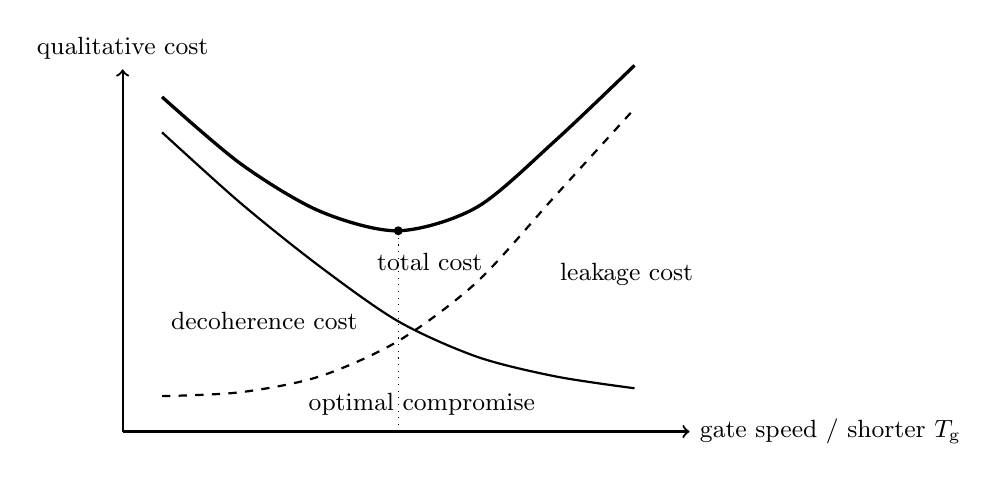
\begin{tikzpicture}[
    x=1cm,y=1cm,
    axis/.style={thick,->},
    curve1/.style={thick},
    curve2/.style={thick,dashed},
    lbl/.style={font=\small}
]

% axes
\draw[axis] (0,0) -- (7.2,0) node[right,lbl] {gate speed / shorter $T_{\mathrm g}$};
\draw[axis] (0,0) -- (0,4.6) node[above,lbl] {qualitative cost};

% coherence cost (decreases with speed)
\draw[curve1]
    plot[smooth] coordinates {(0.5,3.8) (1.5,2.9) (2.5,2.1) (3.5,1.4) (4.5,0.95) (5.5,0.7) (6.5,0.55)};
\node[lbl] at (1.8,1.4) {decoherence cost};

% leakage cost (increases with speed)
\draw[curve2]
    plot[smooth] coordinates {(0.5,0.45) (1.5,0.5) (2.5,0.7) (3.5,1.15) (4.5,1.9) (5.5,3.0) (6.5,4.1)};
\node[lbl] at (6.4,2.0) {leakage cost};

% total cost
\draw[very thick]
    plot[smooth] coordinates {(0.5,4.25) (1.5,3.4) (2.5,2.8) (3.5,2.55) (4.5,2.85) (5.5,3.7) (6.5,4.65)};
\node[lbl] at (3.9,2.15) {total cost};

% optimum marker
\draw[dotted] (3.5,0) -- (3.5,2.55);
\filldraw (3.5,2.55) circle (1.4pt);
\node[lbl] at (3.8,0.35) {optimal compromise};

\end{tikzpicture}
\caption{Qualitative illustration of the speed--leakage tradeoff in weakly anharmonic superconducting qubits. Slower gates suffer more from decoherence and low-frequency noise, whereas faster gates typically increase leakage through stronger driving, broader spectral content, and larger non-adiabatic effects. The physically relevant control problem is therefore a compromise between these competing tendencies.}
\label{fig:speed_leakage_tradeoff}
\end{figure}


% Requires in the preamble:
% \usepackage{amsmath,amssymb,amsfonts,bm}
% \usepackage{tikz}
% \usetikzlibrary{positioning,arrows.meta,fit}
\section{Quantum control theory background}
\subsection{Open-loop and closed-loop quantum control}
\label{subsec:open_closed_loop_control}

A basic conceptual distinction in control theory is that between \emph{open-loop} and \emph{closed-loop} strategies. In an open-loop protocol, the control fields are prescribed in advance and then applied to the system without using measurement outcomes obtained during the same realization of the dynamics. In a closed-loop protocol, by contrast, the controls are adapted using information returned by the system itself, either continuously or iteratively, through some form of measurement and feedback \cite{Koch2022,Ferrie2015,Feng2018}. This distinction is especially important in quantum systems, because measurement is not a passive readout operation: it can introduce statistical uncertainty, backaction, and experimental latency, all of which influence the practicality of feedback-based control. For this reason, the open-loop/closed-loop dichotomy in quantum engineering is both conceptually rich and experimentally consequential.

In the model-based open-loop setting, one begins from a dynamical model
\begin{equation}
\dot{\rho}(t)
=
\mathcal{L}_{\bm{u}(t)}[\rho(t)],
\label{eq:open_loop_dynamics_general}
\end{equation}
where $\rho(t)$ is the quantum state (or density matrix), $\mathcal{L}_{\bm{u}(t)}$ is the generator of the dynamics, and $\bm{u}(t)$ denotes the externally chosen controls. For a closed quantum system this reduces to the Schr\"odinger or von Neumann equation,
\begin{equation}
\dot{\rho}(t)
=
-\frac{i}{\hbar}[H(t;\bm{u}),\rho(t)],
\label{eq:open_loop_vonneumann}
\end{equation}
while in the presence of dissipation one may instead work with a Lindblad generator. The optimization problem is then posed entirely at the level of the model: one selects a parameterized family of controls,
\begin{equation}
\bm{u}(t)=\bm{u}(t;\bm{\theta}),
\label{eq:open_loop_control_parametrization}
\end{equation}
and solves
\begin{equation}
\bm{\theta}^{\star}
=
\arg\min_{\bm{\theta}} \;
\mathcal{J}_{\mathrm{model}}(\bm{\theta}),
\label{eq:open_loop_optimization_problem}
\end{equation}
where $\mathcal{J}_{\mathrm{model}}$ is a model-based objective such as gate infidelity, leakage, runtime, or some weighted combination thereof. Once $\bm{\theta}^{\star}$ has been found numerically, the resulting pulse is implemented experimentally without any intra-shot adaptation. This is the standard framework of much of quantum optimal control, including GRAPE-, Krotov-, GOAT-, and many reinforcement-learning-based approaches when training is performed in simulation \cite{Koch2022}.

The main advantage of open-loop control is that it can exploit a detailed physical model and powerful numerical optimization tools before any experiment is run. It is therefore well suited to platforms for which the Hamiltonian and noise mechanisms are sufficiently well characterized. Moreover, since no measurements are required during the gate execution itself, open-loop control avoids the complications of quantum backaction and avoids the hardware overhead associated with real-time feedback. However, its main weakness is equally clear: the optimized pulse is only as good as the model on which it is based. If the actual device differs significantly from the assumed Hamiltonian, if transfer functions distort the waveform, or if noise sources are incompletely modeled, then a pulse that appears optimal in simulation may perform suboptimally on hardware \cite{Koch2022,Ferrie2015}. This model mismatch is one of the main reasons why purely open-loop design can become unreliable in realistic experiments.

Closed-loop control is introduced precisely to address this gap between model and hardware. In its most literal form, it means that the control applied at time $t_k$ depends on measurement information gathered at earlier times,
\begin{equation}
\bm{u}(t_k)
=
\pi_k\!\left(y_0,y_1,\dots,y_{k-1}\right),
\label{eq:closed_loop_policy}
\end{equation}
where $\{y_j\}$ denotes the measurement record and $\pi_k$ is a control law or feedback policy. In this picture, the system is repeatedly observed and the control is updated in real time according to the observed outcomes. Because quantum measurements disturb the state, such feedback must be described together with the measurement backaction. If $\mathcal{M}_{y}$ denotes the measurement operation associated with outcome $y$, then the post-measurement state is
\begin{equation}
\rho
\;\longmapsto\;
\frac{\mathcal{M}_{y}(\rho)}
{\mathrm{Tr}\!\left[\mathcal{M}_{y}(\rho)\right]},
\label{eq:measurement_backaction}
\end{equation}
with outcome probability
\begin{equation}
p(y)=\mathrm{Tr}\!\left[\mathcal{M}_{y}(\rho)\right].
\label{eq:measurement_probability}
\end{equation}
Thus, unlike in classical control, the act of acquiring information modifies the system whose dynamics one is trying to steer. This makes genuine feedback control more delicate in the quantum regime, especially for fast gate operations where measurement latency and finite measurement fidelity can become serious bottlenecks \cite{Koch2022}.

% \textbf{TODO:} Recheck if I want this in my thesis since

In quantum-information experiments, however, the phrase \emph{closed-loop optimization} is often used in a broader and more practical sense. Rather than updating the control during a single gate execution, one performs repeated experimental shots with a fixed pulse $\bm{u}(t;\bm{\theta}_r)$, estimates a performance metric from the measurement outcomes, and then updates the pulse parameters between shots according to some classical optimization rule. If $\widehat{\mathcal{J}}_{\mathrm{exp}}(\bm{\theta}_r)$ denotes the experimentally estimated cost at iteration $r$, then the iterative update can be written schematically as
\begin{equation}
\bm{\theta}_{r+1}
=
\mathcal{A}
\!\left(
\bm{\theta}_{r},
\widehat{\mathcal{J}}_{\mathrm{exp}}(\bm{\theta}_{r}),
\widehat{\nabla \mathcal{J}}_{\mathrm{exp}}(\bm{\theta}_{r}),
\dots
\right),
\label{eq:iterative_closed_loop_update}
\end{equation}
where $\mathcal{A}$ denotes an optimization rule such as gradient descent, finite-difference search, Bayesian optimization, or a reinforcement-learning policy improvement step. In this experimentally relevant sense, the loop is \emph{closed} not because the Hamiltonian is modified in real time during the gate, but because the control design is iteratively informed by measured performance on the actual device \cite{Ferrie2015,Feng2018}. This distinction is worth stating explicitly, because the words \emph{closed-loop control} may refer either to continuous measurement-based feedback or to shot-to-shot in situ calibration.

The practical strengths of closed-loop approaches are clear. Since the performance metric is measured directly on the physical device, systematic model errors, waveform distortions, and unknown hardware nonlinearities are automatically incorporated into the optimization. This can make closed-loop strategies more robust than purely model-based open-loop methods when the system is imperfectly characterized. Experimental studies indeed show that closed-loop quantum control can outperform open-loop control in settings where model inaccuracies or hardware distortions dominate the error budget \cite{Ferrie2015,Feng2018}. In addition, closed-loop schemes can target figures of merit that are directly operational, such as randomized-benchmarking-based performance estimates or experimentally reconstructed gate fidelities, rather than relying exclusively on idealized simulation objectives.

The price paid for this robustness is experimental cost. Closed-loop methods generally require many repeated measurements, and therefore many experimental iterations, in order to estimate objective functions or gradients with acceptable statistical precision. In fast gate optimization this can become a serious limitation, since readout is often much slower than the gate itself and can perturb subsequent operations. This concern  is emphasized in modern literature: the authors note that many efforts to improve robustness against control errors have focused on closed-loop feedback optimization, but that frequent measurements remain relatively slow and can degrade later fidelities, making such approaches less practical for near-term devices \cite{Niu2019}. In contrast, their approach remains fundamentally open-loop during gate execution, while incorporating robustness and leakage suppression directly into an analytic cost function that can be optimized numerically.

This distinction leads naturally to a hybrid viewpoint. Purely open-loop control is efficient when the model is accurate enough; purely closed-loop control is attractive when the device itself must reveal the relevant imperfections; and many modern workflows combine the two. A common strategy is to first compute a high-quality pulse from a detailed simulation and then refine or calibrate it experimentally through an iterative in situ procedure. Schematically, one may write
\begin{equation}
\bm{\theta}_{0}
=
\arg\min_{\bm{\theta}} \mathcal{J}_{\mathrm{model}}(\bm{\theta}),
\qquad
\bm{\theta}^{\star}
=
\mathrm{Refine}\!\left(
\bm{\theta}_{0},
\widehat{\mathcal{J}}_{\mathrm{exp}}
\right),
\label{eq:hybrid_open_closed_workflow}
\end{equation}
where the first step is model-based and the second experimental. This hybrid logic has become increasingly important in quantum control software and experimental practice, precisely because it attempts to combine the numerical efficiency of open-loop design with the hardware realism of closed-loop refinement \cite{Koch2022,Rossignolo2023}.

For the purposes of this thesis, the most important point is the following. The UFO framework analyzed later is an \emph{open-loop} control framework in the sense that the control pulse is optimized from a Hamiltonian model and then applied without measurement-based feedback during the gate. At the same time, its motivation is shaped by the practical limitations of closed-loop techniques: because repeated measurements are slow and because the exact error model is often unavailable, the framework seeks to encode robustness and leakage suppression directly into the cost function rather than outsourcing them to experimental feedback \cite{Niu2019}. The distinction developed in this subsection is therefore not merely terminological; it explains why the thesis focuses on analytic objectives and model-based control design, while still recognizing that future hardware-level implementations may benefit from hybrid or partially closed-loop refinements.

\begin{figure}[t]
\centering
\begin{tikzpicture}[
    box/.style={draw, rounded corners, minimum width=2.9cm, minimum height=1cm, align=center},
    smallbox/.style={draw, rounded corners, minimum width=2.2cm, minimum height=0.9cm, align=center},
    arrow/.style={-{Latex[length=2mm]}, thick},
    dashedarrow/.style={-{Latex[length=2mm]}, thick, dashed},
    node distance=1.4cm and 1.8cm
]

% OPEN LOOP
% \node[smallbox] (model1) {model / simulator};
\node[smallbox] (model1) {model};
\node[smallbox, right=of model1] (opt1) {optimizer};
\node[smallbox, right=of opt1] (pulse1) {pulse $\bm{u}(t;\bm{\theta}^{\star})$};
\node[smallbox, right=of pulse1] (sys1) {quantum system};

\draw[arrow] (model1) -- (opt1);
\draw[arrow] (opt1) -- (pulse1);
\draw[arrow] (pulse1) -- (sys1);

\node[above=0.3cm of opt1] {\textbf{Open loop}};
\node[below=0.35cm of opt1] {\small no measurement-based update during the gate};

% CLOSED LOOP
\node[smallbox, below=2.3cm of model1] (pulse2) {pulse $\bm{u}(t;\bm{\theta}_r)$};
\node[smallbox, right=of pulse2] (sys2) {quantum system};
\node[smallbox, right=of sys2] (meas2) {measurement \\ and \\ cost estimate};
\node[smallbox, right=of meas2] (opt2) {update rule};

\draw[arrow] (pulse2) -- (sys2);
\draw[arrow] (sys2) -- (meas2);
\draw[arrow] (meas2) -- (opt2);
\draw[dashedarrow] (opt2.north) |- ++(0,1.15) -| (pulse2.north);

\node[above=0.3cm of meas2] {\textbf{Closed loop}};
\node[below=0.35cm of meas2] {\small measured performance updates the next pulse};

\end{tikzpicture}
\caption{Schematic distinction between open-loop and closed-loop quantum control. In open-loop control, pulse design is performed from a model and the resulting pulse is applied without feedback during the gate. In closed-loop control, experimental information is fed back to improve the next control decision, either in real time or iteratively between repeated runs.}
\label{fig:open_closed_loop_control}
\end{figure}

\subsection{Classical optimal-control methods for quantum systems}
\label{subsec:classical_qoc_methods}

Before introducing reinforcement-learning-based control, it is useful to summarize the main families of \emph{classical} optimal-control methods that have shaped modern quantum pulse engineering. In all of them, the basic problem is the same: one specifies a dynamical model, chooses a parameterization of the control fields, defines a cost functional that encodes the target task, and then numerically optimizes the control so as to minimize that cost \cite{Khaneja2005,Palao2003,Reich2012,Caneva2011,Machnes2018}. These methods are typically \emph{open-loop} and \emph{model-based}: they rely on repeated simulation of the controlled Schr\"odinger or Lindblad dynamics, and they assume that the model captures the relevant physics with sufficient fidelity.

A general quantum optimal-control problem can be written as follows. Let the system dynamics be governed by a controlled Hamiltonian
\begin{equation}
H(t;\bm{u})
=
H_{\mathrm{d}}
+
\sum_{k=1}^{m} u_k(t)\,H_k,
\label{eq:qoc_controlled_hamiltonian}
\end{equation}
with propagator $U(t)$ satisfying
\begin{equation}
i\hbar \frac{d}{dt} U(t)
=
H(t;\bm{u})\,U(t),
\qquad
U(0)=\mathbb{I}.
\label{eq:qoc_propagator_equation}
\end{equation}
The optimization objective is encoded in a cost functional of the generic form
\begin{equation}
\mathcal{J}[\bm{u}]
=
\Phi\!\bigl(U(T)\bigr)
+
\int_{0}^{T} g\!\bigl(\bm{u}(t),t\bigr)\,dt,
\label{eq:qoc_cost_functional}
\end{equation}
where $\Phi$ is a terminal cost, for example a gate-infidelity or state-transfer error, and $g$ is a running cost encoding penalties such as pulse energy, smoothness, boundary conditions, or robustness terms. In practice the control is often discretized on a time grid
\begin{equation}
u_k(t)=u_{k,\ell},
\qquad
t\in[t_\ell,t_{\ell+1}),
\qquad
\ell=0,\dots,N-1,
\label{eq:qoc_piecewise_constant}
\end{equation}
which reduces the infinite-dimensional search problem to a finite-dimensional optimization over the amplitudes $\{u_{k,\ell}\}$.

One of the most influential methods in this setting is \emph{GRAPE} (Gradient Ascent Pulse Engineering), originally developed in the NMR community and later widely adopted in quantum information processing \cite{Khaneja2005,deFouquieres2011}. The central idea of GRAPE is to compute the gradient of the cost functional with respect to each control amplitude $u_{k,\ell}$ efficiently by combining forward propagation of the state or propagator with backward propagation of an adjoint variable. In its simplest gradient-descent or gradient-ascent form, the update reads
\begin{equation}
u_{k,\ell}^{(r+1)}
=
u_{k,\ell}^{(r)}
-
\eta
\frac{\partial \mathcal{J}}{\partial u_{k,\ell}},
\label{eq:grape_update}
\end{equation}
where $\eta$ is a step size and $r$ indexes the optimization iteration. The practical strength of GRAPE is that all control amplitudes can be optimized simultaneously with gradients that scale efficiently once the forward and backward trajectories have been computed. This makes it especially powerful for high-dimensional pulse optimization with fine time discretization.

For state-transfer objectives, the structure of the GRAPE gradient can be illustrated in a standard bilinear setting. Let $\ket{\psi_\ell}$ be the forward-propagated state at time step $\ell$ and let $\ket{\chi_{\ell+1}}$ be the corresponding backward-propagated adjoint state. Then the gradient contribution of the control amplitude $u_{k,\ell}$ has the generic form
\begin{equation}
\frac{\partial \mathcal{J}}{\partial u_{k,\ell}}
\propto
-\operatorname{Im}
\left\langle
\chi_{\ell+1}
\middle|
H_k
\middle|
\psi_\ell
\right\rangle,
\label{eq:grape_gradient_generic}
\end{equation}
up to convention-dependent prefactors and discretization factors. Equation~\eqref{eq:grape_gradient_generic} makes clear why GRAPE is computationally attractive: all gradients are obtained from quantities already available during propagation. Later refinements, such as second-order GRAPE and quasi-Newton acceleration, improve convergence speed and numerical robustness without changing this core adjoint-based structure \cite{deFouquieres2011}.

A second major family is based on \emph{Krotov-type} updates. In the quantum-control literature, Krotov's method is valued for its variational foundation and for the possibility of obtaining \emph{monotonic convergence}, meaning that the objective improves at every iteration under appropriate assumptions \cite{Palao2003,Reich2012}. Instead of viewing the optimization merely as a local gradient step in a large Euclidean parameter space, Krotov's method constructs an update directly from the stationarity conditions of the augmented control functional. In a common first-order setting, one obtains an update of the form
\begin{equation}
u_k^{(r+1)}(t)
=
u_k^{(r)}(t)
+
\frac{S_k(t)}{\lambda_k}
\,\operatorname{Im}
\left\langle
\chi^{(r)}(t)
\middle|
\frac{\partial H}{\partial u_k}
\middle|
\psi^{(r+1)}(t)
\right\rangle,
\label{eq:krotov_update}
\end{equation}
where $S_k(t)$ is a shape function enforcing boundary smoothness or turn-on/turn-off constraints, $\lambda_k$ is a step-size-like penalty parameter, and $\ket{\chi^{(r)}(t)}$ and $\ket{\psi^{(r+1)}(t)}$ are the adjoint and forward states associated with consecutive iterations. The characteristic feature of Eq.~\eqref{eq:krotov_update} is that the new control depends on the newly propagated state $\ket{\psi^{(r+1)}(t)}$, which is one reason why Krotov-type schemes differ structurally from straightforward GRAPE updates.

While GRAPE and Krotov are both gradient-based, they differ in philosophy and practical use. GRAPE is often especially convenient when the controls are piecewise constant and when one wishes to use standard unconstrained optimization tools such as BFGS or L-BFGS in a high-dimensional parameter space. Krotov's method is often preferred when monotonic convergence, time-dependent constraints, or specific functional forms of the objective are important. Both, however, belong to the same broad class: they optimize a cost functional by exploiting gradient information computed from the controlled dynamics \cite{Khaneja2005,Reich2012}.

A rather different strategy is embodied by \emph{CRAB} (Chopped Random Basis), which reduces the search space by expanding the control in a truncated basis and optimizing only the corresponding coefficients \cite{Caneva2011}. A typical CRAB parameterization reads
\begin{equation}
u_k(t)
=
u_k^{(0)}(t)
\left[
1+
\sum_{m=1}^{M}
\left(
A_{k,m}\sin \omega_{k,m} t
+
B_{k,m}\cos \omega_{k,m} t
\right)
\right],
\label{eq:crab_ansatz}
\end{equation}
where $u_k^{(0)}(t)$ is a reference pulse, the frequencies $\omega_{k,m}$ are chosen or randomized within a suitable range, and the coefficients $A_{k,m},B_{k,m}$ become the optimization variables. The conceptual advantage is clear: instead of optimizing hundreds or thousands of piecewise-constant amplitudes, one works in a much lower-dimensional space of coefficients that can naturally encode smoothness, bandwidth restrictions, and experimental simplicity. Because of this reduced parametrization, CRAB is particularly useful when gradients are expensive or unavailable, and it is often combined with gradient-free optimizers such as Nelder--Mead or simplex-type search strategies \cite{Caneva2011}. This basis-restricted perspective is also attractive in experimental closed-loop refinements, where each additional optimization variable may carry a substantial measurement cost.

\textbf{TODO:} Decidere se voglio tenere Goat e krotov

A more recent method that addresses some of the limitations of both piecewise-constant gradient methods and purely gradient-free basis search is \emph{GOAT} (Gradient Optimization of Analytic conTrols) \cite{Machnes2018}. The guiding idea of GOAT is to keep the controls in a low-dimensional but analytic parameterization,
\begin{equation}
u_k(t)=u_k(t;\bm{\theta}),
\label{eq:goat_analytic_controls}
\end{equation}
and to compute exact gradients with respect to the parameters $\bm{\theta}$ by propagating not only the system evolution but also its derivatives. If $U(t;\bm{\theta})$ denotes the propagator, then differentiation of Eq.~\eqref{eq:qoc_propagator_equation} with respect to a parameter $\theta_j$ yields the coupled evolution equation
\begin{equation}
i\hbar \frac{d}{dt}
\left(
\frac{\partial U}{\partial \theta_j}
\right)
=
H(t;\bm{\theta})
\frac{\partial U}{\partial \theta_j}
+
\frac{\partial H(t;\bm{\theta})}{\partial \theta_j}
U(t;\bm{\theta}),
\label{eq:goat_derivative_equation}
\end{equation}
with initial condition
\begin{equation}
\frac{\partial U(0;\bm{\theta})}{\partial \theta_j}=0.
\label{eq:goat_derivative_initial}
\end{equation}
Thus, once the augmented system formed by $U$ and its derivatives is propagated, one obtains the gradient of the final cost $\partial \mathcal{J}/\partial \theta_j$ directly. The principal appeal of GOAT is that it combines gradient efficiency with flexible, low-dimensional, hardware-friendly pulse parametrizations, making it particularly attractive for superconducting qubits where pulse simplicity and subsequent experimental calibration matter greatly \cite{Machnes2018}.

From a broader perspective, GRAPE, Krotov, CRAB, and GOAT should not be viewed as mutually exclusive competitors so much as different design philosophies for the same underlying problem. GRAPE and Krotov prioritize gradient information and direct optimization in control space; CRAB prioritizes dimensional reduction and basis flexibility; GOAT attempts to retain exact gradients while working in a compact analytic parameter space. The best method depends on the physics, the size of the system, the availability of gradients, the presence of constraints, and whether the pulse will later need to be calibrated on hardware \cite{Khaneja2005,Caneva2011,Machnes2018}. In superconducting circuits, for example, piecewise-constant pulses may be numerically convenient but experimentally awkward, while smooth low-parameter pulses may be easier to calibrate and less sensitive to transfer-function distortions.

For the purposes of this thesis, these methods serve two roles. First, they provide the standard background language of open-loop model-based quantum control: objective functional, parameterization, gradient computation, and iterative pulse improvement. Second, they define the natural baseline against which reinforcement-learning-based methods should be interpreted. Reinforcement learning does not replace the optimal-control problem itself; rather, it offers an alternative way to search the space of control laws, especially in settings where the cost landscape is highly nonconvex, robustness matters strongly, or sequential structure can be exploited. The value of the approach studied in the reference paper is therefore best understood not in isolation, but against the mature backdrop of these classical optimal-control techniques.

% Optional compact summary equation
% It is useful to summarize the common structure of all these methods schematically as
% \begin{equation}
% \text{model}
% \;+\;
% \text{control ansatz}
% \;+\;
% \text{cost functional}
% \;+\;
% \text{numerical optimizer}
% \;\longrightarrow\;
% \text{optimized pulse}.
% \label{eq:qoc_common_pipeline}
% \end{equation}
% What distinguishes GRAPE, Krotov, CRAB, and GOAT is not the overall control objective, but the specific choice of control ansatz, gradient computation, and update rule used to navigate the optimization landscape.


\subsection{Why robustness is difficult in quantum control}
\label{subsec:why_robustness_is_difficult}

In an idealized optimal-control problem one assumes that the system Hamiltonian, the control transfer function, and the relevant noise model are all known accurately. Under these assumptions, one can optimize a pulse for a \emph{nominal} model and obtain extremely high fidelities in simulation. In practice, however, quantum control is almost never deployed under such perfectly known conditions. Device parameters drift, couplings are incompletely calibrated, control electronics distort the intended waveform, environmental noise is only partially characterized, and higher-level dynamics may not be fully captured by the chosen effective model. As a result, a pulse that is optimal for a nominal model may perform poorly once implemented on the actual device \cite{Koch2022,Weidner2025,Propson2022}. This gap between nominal optimality and physical reliability is the basic reason robustness is difficult.

A convenient way to formalize this point is to write the dynamics as depending not only on the control $\bm{u}(t)$ but also on uncertain parameters $\bm{\delta}$:
\begin{equation}
\dot{\rho}(t)
=
\mathcal{L}_{\bm{u}(t),\,\bm{\delta}}[\rho(t)].
\label{eq:uncertain_quantum_dynamics}
\end{equation}
Here $\bm{\delta}$ may represent static detuning errors, drift in anharmonicity, imprecise couplings, control-amplitude distortions, fluctuating calibration offsets, or environmental parameters. If one defines a nominal performance functional $\mathcal{J}(\bm{u};\bm{\delta})$, then the standard open-loop optimization problem corresponds to minimizing
\begin{equation}
\mathcal{J}_{\mathrm{nom}}(\bm{u})
:=
\mathcal{J}(\bm{u};\bm{\delta}_{0}),
\label{eq:nominal_cost}
\end{equation}
for a single reference value $\bm{\delta}_0$. A robust-control problem, by contrast, must account for a whole \emph{set} or \emph{distribution} of possible uncertainties. This immediately makes the problem more difficult, because the optimizer is no longer asked to perform well at one point in parameter space, but over a family of models.

There are several inequivalent ways to formulate robustness. In an \emph{average-case} formulation one assumes that the uncertainty is drawn from a probability distribution $p(\bm{\delta})$ and optimizes the expected cost
\begin{equation}
\mathcal{J}_{\mathrm{avg}}(\bm{u})
=
\mathbb{E}_{\bm{\delta}\sim p}
\left[
\mathcal{J}(\bm{u};\bm{\delta})
\right]
=
\int
\mathcal{J}(\bm{u};\bm{\delta})\,
p(\bm{\delta})\,d\bm{\delta}.
\label{eq:average_case_robustness}
\end{equation}
In a \emph{worst-case} or minimax formulation one instead seeks to control the largest possible degradation over an uncertainty set $\Delta$:
\begin{equation}
\mathcal{J}_{\mathrm{wc}}(\bm{u})
=
\sup_{\bm{\delta}\in\Delta}
\mathcal{J}(\bm{u};\bm{\delta}).
\label{eq:worst_case_robustness}
\end{equation}
A third common viewpoint is threshold-based, where one requires the fidelity or success probability to remain above a prescribed level with high probability:
\begin{equation}
\mathbb{P}_{\bm{\delta}\sim p}
\!\left(
F(\bm{u};\bm{\delta}) \geq F_{\min}
\right)
\geq 1-\varepsilon.
\label{eq:chance_constraint_robustness}
\end{equation}
These three criteria encode genuinely different priorities. A control that is excellent on average can still fail badly on rare but important perturbations, while a minimax-optimal control may be too conservative for average experimental operation \cite{Weidner2025,Propson2022}. Thus, robustness is not a single scalar property but a design choice that depends on what failure modes one wishes to suppress.

A second source of difficulty is that the uncertainty set itself is often only partially known. In many experiments one does not know the exact noise law $p(\bm{\delta})$, and even if some approximate characterization is available, it may drift in time. This issue is explicitly emphasized in the literature, where the authors note that the exact model of control errors is often unavailable and may vary over time, so that one should ideally seek control strategies that remain reliable not merely for one precisely specified perturbation model, but across a broader family of experimentally relevant error processes \cite{Niu2019}. Formally, this means that one often trains or optimizes under one distribution $p_{\mathrm{train}}(\bm{\delta})$ while the actual deployment conditions follow another distribution $p_{\mathrm{deploy}}(\bm{\delta})$, with
\begin{equation}
p_{\mathrm{train}}(\bm{\delta})
\neq
p_{\mathrm{deploy}}(\bm{\delta}).
\label{eq:distribution_shift}
\end{equation}
Equation~\eqref{eq:distribution_shift} is the control-theoretic version of distribution shift: a pulse may appear robust in simulation but degrade under out-of-distribution perturbations that were absent or underrepresented during optimization.

A third difficulty is computational. To evaluate the nominal objective in Eq.~\eqref{eq:nominal_cost}, one usually needs only a single propagation of the system dynamics per iteration. By contrast, evaluating a robust objective typically requires many propagations over different uncertainty realizations or uncertainty-grid points. If one approximates the average-case objective by Monte Carlo sampling with $M$ samples,
\begin{equation}
\mathcal{J}_{\mathrm{avg}}(\bm{u})
\approx
\frac{1}{M}
\sum_{j=1}^{M}
\mathcal{J}(\bm{u};\bm{\delta}^{(j)}),
\label{eq:monte_carlo_robustness}
\end{equation}
then every optimization step becomes roughly $M$ times more expensive than the nominal one. This sampling burden can become severe in multi-qubit systems, especially when the control space is already high-dimensional. The difficulty is compounded when one wishes to include realistic open-system evolution, since each propagation may then require solving a Lindblad master equation rather than a closed-system Schr\"odinger equation \cite{Weidner2025,Propson2022,Goldschmidt2022}. Robustness is therefore not hard only because of physics; it is hard because it is computationally expensive to certify.

A fourth source of difficulty is geometric. The control landscape of a nominal problem is already high-dimensional and nonconvex. Introducing robustness means that the optimizer must now navigate not one landscape, but an \emph{aggregate} landscape produced by averaging or extremizing over many perturbations. Even if each individual cost $\mathcal{J}(\bm{u};\bm{\delta})$ were relatively benign, their superposition can produce a far more intricate structure with flatter regions, competing descent directions, and stronger tradeoffs between objectives. In local sensitivity analysis one may expand the cost around a nominal control $\bm{u}_{0}$ as
\begin{equation}
\mathcal{J}(\bm{u}_{0}+\Delta \bm{u})
\approx
\mathcal{J}(\bm{u}_{0})
+
\nabla \mathcal{J}(\bm{u}_{0})^{\top}\Delta \bm{u}
+
\frac{1}{2}\Delta \bm{u}^{\top}
H_{\mathcal{J}}(\bm{u}_{0})
\Delta \bm{u},
\label{eq:hessian_expansion_robustness}
\end{equation}
where $H_{\mathcal{J}}$ is the Hessian of the control objective. Robustness analysis based on such curvature information can be very informative, because it quantifies sensitivity to small perturbations in the controls. But it is also expensive in large systems: as the literature points out, canonical Hessian-based robustness analysis becomes computationally prohibitive as the number of control degrees of freedom grows, which is one reason the authors adopt a more scalable practical robustness definition \cite{Niu2019}. Thus, even diagnosing whether a pulse is robust can already be difficult, before one attempts to optimize robustness itself.

Another complication is that different sources of robustness may conflict with one another. A control that is robust against amplitude noise may be fragile against detuning error; a control that is robust against quasistatic drift may be more sensitive to bandwidth truncation; a pulse that suppresses leakage may require longer duration and thus suffer more strongly from decoherence. In this sense, robustness is not usually a single-axis improvement but a multidimensional tradeoff problem. A more realistic objective is therefore often of the form
\begin{equation}
\mathcal{J}_{\mathrm{rob}}[\bm{u}]
=
w_{F}\,\varepsilon_{\mathrm{gate}}
+
w_{L}\,L
+
w_{T}\,T
+
w_{R}\,\mathcal{R}[\bm{u}],
\label{eq:multiobjective_robustness}
\end{equation}
where $\mathcal{R}[\bm{u}]$ denotes a chosen robustness functional and the weights $\{w_F,w_L,w_T,w_R\}$ encode the tradeoff between fidelity, leakage, runtime, and robustness. There is generally no reason for these objectives to be simultaneously minimized by the same pulse. A robust-control problem is therefore often a Pareto problem rather than a single-objective one.

In superconducting qubits, the robustness problem is made sharper by the multilevel character of the hardware. Parameter uncertainty does not merely perturb the logical gate within the computational subspace; it can alter detunings, anharmonicities, and couplings in a way that changes the leakage channels themselves. Thus, robustness against model uncertainty and robustness against leakage are intertwined rather than separable. This is one reason why robust pulse design in weakly anharmonic systems often requires the full multilevel Hamiltonian rather than a simplified two-level approximation \cite{Krantz2019,Propson2022}. The same observation is directly relevant for the reference paper: its robust RL optimization is performed in a stochastic environment where perturbations are injected into physically important control parameters, and the resulting performance is then judged by averaged noisy gate fidelity and fidelity variance rather than by nominal accuracy alone \cite{Niu2019}.

It is therefore useful to distinguish two questions:
\begin{enumerate}
\item \emph{Robustness evaluation:} given a control pulse, how sensitive is it to perturbations?
\item \emph{Robustness optimization:} how should the pulse be modified so as to reduce that sensitivity?
\end{enumerate}
The first is already nontrivial because it requires specifying the relevant uncertainty model and computing the corresponding sensitivity metric. The second is harder still because robustness must be optimized jointly with all the other physical criteria of the control problem. In that sense, robustness is difficult not because it is a secondary correction to nominal control, but because it fundamentally changes the optimization problem itself.

For the purposes of this thesis, the most important takeaway is that robustness cannot be treated as an afterthought. A pulse optimized only for nominal gate fidelity may be scientifically interesting, but it is not yet a practically convincing control solution unless one also understands how it behaves under uncertainty, noise, and imperfect modeling. This is precisely why the literature moves beyond a purely nominal objective and evaluates control performance under a family of stochastic perturbations, using average fidelity and fidelity variance as practical diagnostics of robustness \cite{Niu2019}. The extension work proposed later in this thesis builds directly on this point by asking whether robustness learned under one uncertainty model generalizes to others.

\begin{figure}[t]
\centering
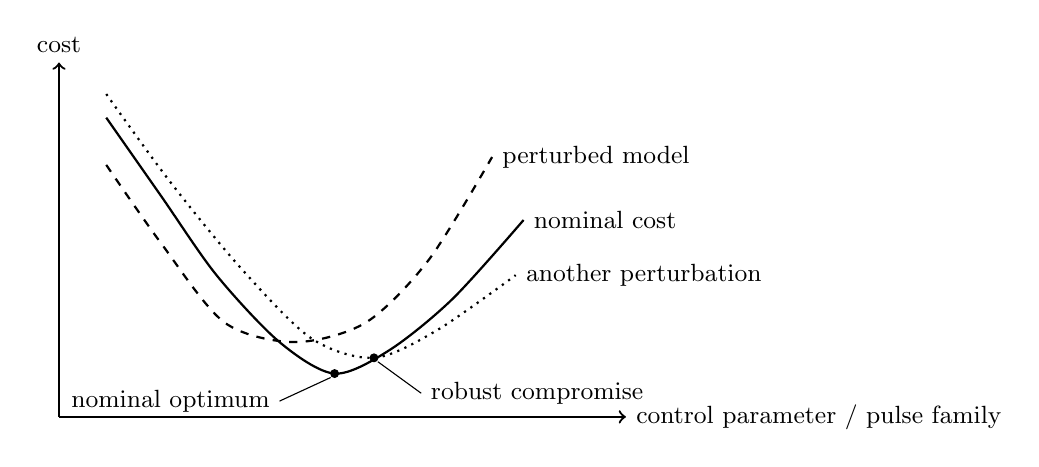
\begin{tikzpicture}[
    axis/.style={thick,->},
    curve/.style={thick},
    lbl/.style={font=\small}
]

% axes
\draw[axis] (0,0) -- (7.2,0) node[right,lbl] {control parameter / pulse family};
\draw[axis] (0,0) -- (0,4.5) node[above,lbl] {cost};

% nominal cost
\draw[curve]
    plot[smooth] coordinates {(0.6,3.8) (1.3,2.8) (2.0,1.8) (2.8,0.95) (3.5,0.55) (4.2,0.85) (5.0,1.5) (5.9,2.5)}
    node[right,lbl] {nominal cost};

% perturbed cost 1
\draw[curve,dashed]
    plot[smooth] coordinates {(0.6,3.2) (1.3,2.2) (2.1,1.2) (3.0,0.95) (3.9,1.2) (4.7,2.0) (5.5,3.3)}
    node[right,lbl] {perturbed model};

% perturbed cost 2
\draw[curve,dotted]
    plot[smooth] coordinates {(0.6,4.1) (1.4,3.0) (2.3,1.9) (3.2,1.0) (4.0,0.75) (4.8,1.1) (5.8,1.8)}
    node[right,lbl] {another perturbation};

% markers
\filldraw (3.5,0.55) circle (1.4pt);
\draw[thin] (3.45,0.5) -- (2.8,0.2) node[left, lbl] {nominal optimum};

\filldraw (4.0,0.75) circle (1.4pt);
\draw[thin] (4.05,0.7) -- (4.6,0.3) node[right, lbl] {robust compromise};

\end{tikzpicture}
\caption{Schematic illustration of why robustness is difficult. A pulse that is optimal for a nominal model need not remain optimal when the Hamiltonian, noise parameters, or control transfer functions are perturbed. Robust optimization must account for an ensemble of such landscapes rather than for a single nominal one.}
\label{fig:robustness_landscape_shift}
\end{figure}

\section{Machine learning and RL for control}
\subsection{Why reinforcement learning is relevant for quantum control}
\label{subsec:why_rl_is_relevant}

Reinforcement learning (RL) is relevant to quantum control because many pulse-design problems are naturally sequential, stochastic, high-dimensional, and lack labeled training data. In contrast to supervised learning, where one learns from example input-output pairs, RL learns by trial and error through repeated interaction with an environment and by maximizing a scalar reward signal \cite{SuttonBarto2018,Giannelli2022}. This makes it appealing for quantum-control settings in which one can evaluate the quality of a control protocol through simulation or experiment, but cannot provide a database of known optimal pulses in advance. The reference paper studied in this thesis emphasizes precisely this point: in the presence of leakage, control noise, and poorly understood high-dimensional control landscapes, RL offers a flexible framework for learning good control trajectories directly from the optimization objective rather than from labeled data \cite{Niu2019}.

At a formal level, RL models the control task as a Markov decision process (MDP), specified by a state space $\mathcal{S}$, an action space $\mathcal{A}$, a transition kernel $P(s'|s,a)$, and a reward function $r(s,a,s')$. At discrete time step $t$, the agent observes a state $s_t\in\mathcal{S}$, selects an action $a_t\in\mathcal{A}$ according to a policy $\pi_{\bm{\theta}}(a|s)$ parameterized by $\bm{\theta}$, receives a reward $r_t$, and transitions to a new state $s_{t+1}$. The cumulative performance of the policy is quantified through the return
\begin{equation}
G_t
=
\sum_{k=t}^{T}
\gamma^{\,k-t} r_k,
\label{eq:rl_return}
\end{equation}
where $\gamma\in[0,1]$ is the discount factor and $T$ is the horizon of an episode. The learning objective is then
\begin{equation}
J(\pi_{\bm{\theta}})
=
\mathbb{E}_{\tau\sim \pi_{\bm{\theta}},P}
\left[
G_0
\right],
\label{eq:rl_objective}
\end{equation}
where the expectation is taken over trajectories
\begin{equation}
\tau
=
(s_0,a_0,r_0,s_1,a_1,r_1,\dots,s_T).
\label{eq:rl_trajectory}
\end{equation}
In words, the agent seeks a policy that maximizes expected cumulative reward over entire control episodes \cite{SuttonBarto2018}.

This formalism maps naturally onto quantum control. The \emph{state} may encode the current time step, the propagated wavefunction or density matrix, effective features derived from the system state, or a partial measurement record in a feedback setting. The \emph{action} corresponds to the control values applied over the next time interval, for example a vector of microwave amplitudes, phases, or detunings. The \emph{environment} is the controlled quantum system itself, either simulated numerically or accessed experimentally. The \emph{reward} is derived from the control objective, such as gate fidelity, state-transfer fidelity, leakage suppression, runtime penalties, or some weighted combination thereof. Thus, quantum pulse design can be interpreted as a sequential decision problem in which the agent gradually constructs a control protocol while observing its consequences through the system dynamics \cite{Giannelli2022,Bukov2018,Niu2019}.

A particularly useful feature of the RL perspective is that it unifies open-loop and closed-loop control under the same conceptual language. If the state contains only the time index,
\begin{equation}
s_t = t,
\label{eq:time_only_state}
\end{equation}
then the learned policy
\begin{equation}
a_t = \pi_{\bm{\theta}}(t)
\label{eq:open_loop_rl_policy}
\end{equation}
defines an effectively open-loop pulse schedule: the action at time $t$ is predetermined once the policy parameters are fixed. If, on the other hand, the state includes a measurement history or experimentally observed features,
\begin{equation}
s_t = \bigl(t,y_0,y_1,\dots,y_{t-1}\bigr),
\label{eq:feedback_state_rl}
\end{equation}
then the same policy formalism becomes a closed-loop feedback controller. This flexibility is one reason RL has become attractive in quantum technologies: it can be used both to learn open-loop pulse sequences and, at least in principle, to learn adaptive feedback strategies within a single mathematical framework \cite{SuttonBarto2018,Giannelli2022}.

Another reason RL is relevant is that many quantum-control objectives are naturally \emph{delayed}. A control action applied early in the pulse sequence may only reveal its true value at the final time, when fidelity, leakage, or some other terminal metric is evaluated. In such cases, it is often convenient to use a reward structure of the form
\begin{equation}
r_t =
\begin{cases}
0, & t<T,\\[0.3em]
-\mathcal{J}_{\mathrm{final}}, & t=T,
\end{cases}
\label{eq:sparse_terminal_reward}
\end{equation}
or, equivalently, a positive terminal reward based on fidelity,
\begin{equation}
r_T = F_{\mathrm{final}}.
\label{eq:terminal_fidelity_reward}
\end{equation}
This sparse-reward structure is awkward for naive local optimization, but it is entirely natural in RL, where the goal is to learn sequences of actions whose value may only become apparent at the end of the episode. In this sense, RL is well suited to control problems in which the quality of a full pulse sequence matters more than the immediate effect of each individual control action \cite{Bukov2018,Giannelli2022}.

RL is also attractive when stochasticity is intrinsic to the problem. If the environment contains random perturbations, sampled parameter drifts, or control noise, then the transition law becomes stochastic,
\begin{equation}
s_{t+1} \sim P(\,\cdot \mid s_t,a_t,\xi_t),
\label{eq:stochastic_transition_rl}
\end{equation}
where $\xi_t$ represents a random disturbance. The policy objective in Eq.~\eqref{eq:rl_objective} then automatically becomes an expectation over noisy trajectories. This is a particularly natural way to formulate robust control: instead of first optimizing a nominal pulse and then testing it under perturbations, one can train the agent directly in a noisy environment and thereby encourage the policy to discover actions that perform well \emph{on average} across many stochastic realizations \cite{Niu2019}. 
This thesis uses exactly this principle by training RL agents in environments with sampled control noise so as to optimize not only fidelity and runtime, but also robustness against stochastic control errors.

A further advantage of RL is that it can exploit structure beyond local differential information. Classical gradient-based optimal control methods often update a pulse by using local derivatives of a cost functional with respect to control parameters. RL, by contrast, can treat the control problem as a long-horizon sequential optimization problem and may therefore exploit nonlocal regularities of the trajectory space. This perspective has been particularly fruitful in problems where the control landscape is highly nonconvex or where the action sequence has strong temporal dependencies. The literature stresses this point explicitly, arguing that deep RL can harness nonlocal regularities of noisy control trajectories and facilitate transfer learning between related control tasks \cite{Niu2019}. This is especially relevant for families of quantum gates that share common structure, because a learned policy or value representation may generalize across nearby targets better than a pulse optimized from scratch each time.

Of course, RL is not automatically superior to classical optimal control. It introduces its own challenges: large sample requirements, sensitivity to reward shaping, instability during training, and the need to choose a suitable state representation and action parameterization. In addition, many RL algorithms were originally developed for generic machine-learning tasks rather than for the special structure of quantum dynamics. For this reason, a productive viewpoint is not to see RL as replacing optimal control, but rather as providing an alternative search strategy within the same control-theoretic framework \cite{Giannelli2022,Bukov2018}. In deterministic model-based settings, RL may be interpreted as learning to solve the same optimization problem attacked by GRAPE or Krotov, but by optimizing a policy over sequential decisions rather than directly differentiating a cost with respect to a fixed pulse vector.

For the purposes of this thesis, the relevance of RL is therefore twofold. First, it offers a mathematically natural framework for sequential pulse construction in noisy and uncertain environments. Second, it provides a route to incorporating practical objectives such as leakage suppression, robustness to sampled perturbations, and gate-time reduction into a single reward function. This is precisely the role RL plays in the UFO framework analyzed later: the control problem is cast as a sequential decision process, the total objective is encoded into a reward/cost signal, and the agent learns pulse trajectories that balance fidelity, leakage, runtime, and robustness under stochastic control errors as it will be covered in section \ref{subsec:ufo_cost_function}. In this sense, RL is relevant not because quantum control is a machine-learning problem in disguise, but because the structure of many realistic quantum-control tasks already has the architecture of a sequential decision problem.

\begin{figure}[t]
\centering
\begin{tikzpicture}[
    box/.style={draw, rounded corners, minimum width=3.0cm, minimum height=1.0cm, align=center},
    arrow/.style={-{Latex[length=2mm]}, thick},
    node distance=1.8cm and 1.8cm
]

\node[box] (agent) {RL agent\\policy $\pi_{\bm{\theta}}(a|s)$};
\node[box, right=of agent] (env) {quantum environment\\Hamiltonian dynamics + noise};
\node[box, below=of env] (reward) {reward / cost\\fidelity, leakage, runtime};
\node[box, below=of agent] (state) {state representation\\time, observables, history};

\draw[arrow] (agent) -- node[above] {$a_t$} (env);
\draw[arrow] (env) -- node[right] {$r_t$} (reward);
\draw[arrow] (reward) -- ++(-3.35,0) |- (agent);
\draw[arrow] (env) -- node[left] {$s_{t+1}$} (state);
\draw[arrow] (state) -- (agent);

\end{tikzpicture}
\caption{Agent--environment view of quantum control in reinforcement learning. The agent chooses control actions, the quantum system evolves under those controls and possible noise, and the resulting state and reward are fed back to improve the policy. Depending on the choice of state representation, the same formalism can describe either open-loop pulse generation or closed-loop feedback control.}
\label{fig:rl_quantum_control_loop}
\end{figure}

\subsection{Policy optimization for continuous-action quantum control}
\label{subsec:policy_optimization_continuous_actions}

Once a quantum-control task has been formulated as a sequential decision problem, the next issue is how the policy should be represented and optimized. This question is especially important in pulse engineering, because the controls applied to a quantum device are typically \emph{continuous} variables: microwave amplitudes, phases, detunings, and coupler biases take values in subsets of $\mathbb{R}^{m}$ rather than in a small discrete action set. For this reason, many quantum-control problems are more naturally approached with \emph{policy optimization} methods than with purely value-based reinforcement-learning algorithms originally designed for discrete actions \cite{SuttonBarto2018,Silver2014,Giannelli2022}. The reference paper studied in this thesis fits exactly into this setting: at each time step, the agent chooses continuous control values, and the resulting pulse trajectory is optimized through a policy-gradient method, specifically trust-region policy optimization (TRPO) \cite{Niu2019}.

To make this precise, let the control horizon be divided into discrete time steps $t=0,1,\dots,T-1$, and let the action at time $t$ be a continuous vector
\begin{equation}
a_t \in \mathcal{A} \subseteq \mathbb{R}^{m}.
\label{eq:continuous_action_space}
\end{equation}
In the context of quantum pulse design, one may identify
\begin{equation}
a_t \equiv \bm{u}_t,
\label{eq:action_as_control_vector}
\end{equation}
where $\bm{u}_t$ denotes the set of control amplitudes applied over the next time slice. A parameterized stochastic policy then specifies a probability density over actions conditioned on the current state:
\begin{equation}
a_t \sim \pi_{\bm{\theta}}(\,\cdot \mid s_t),
\label{eq:stochastic_policy_sampling}
\end{equation}
with parameters $\bm{\theta}$. In continuous-control applications, a common choice is a Gaussian policy,
\begin{equation}
\pi_{\bm{\theta}}(a\mid s)
=
\mathcal{N}\!\bigl(a;\,\bm{\mu}_{\bm{\theta}}(s),\,\Sigma_{\bm{\theta}}(s)\bigr),
\label{eq:gaussian_policy}
\end{equation}
where $\bm{\mu}_{\bm{\theta}}(s)$ is the policy mean and $\Sigma_{\bm{\theta}}(s)$ is the covariance matrix. Equation~\eqref{eq:gaussian_policy} is particularly natural for pulse optimization, because it allows the policy to output a mean control action together with an exploration scale, thereby balancing exploitation of already promising pulse shapes with continued sampling of nearby alternatives \cite{SuttonBarto2018,Schulman2015}.

The fundamental reason policy methods are attractive in this setting is that value-based action maximization becomes awkward in continuous spaces. In discrete-action reinforcement learning, a greedy policy can be obtained by choosing
\begin{equation}
a^{\star}(s)
=
\arg\max_{a\in\mathcal{A}} Q(s,a),
\label{eq:discrete_greedy_action}
\end{equation}
since the maximization involves only finitely many candidate actions. In continuous spaces, however, the analogous operation
\begin{equation}
a^{\star}(s)
=
\arg\max_{a\in\mathbb{R}^{m}} Q(s,a)
\label{eq:continuous_action_maximization}
\end{equation}
is itself a nontrivial optimization problem that must, in principle, be solved at every time step. This greatly complicates the use of purely value-based methods in continuous-control domains. Policy optimization avoids this issue by directly parameterizing the control law $a=\pi_{\bm{\theta}}(s)$ or the action density $\pi_{\bm{\theta}}(a\mid s)$ and updating its parameters to improve the expected return \cite{Silver2014,SuttonBarto2018}. For quantum control, where the action is already the pulse amplitude vector, this direct parameterization is especially natural.

The objective remains the expected discounted return,
\begin{equation}
J(\bm{\theta})
=
\mathbb{E}_{\tau\sim\pi_{\bm{\theta}}}
\left[
\sum_{t=0}^{T}
\gamma^{t} r_t
\right],
\label{eq:policy_objective_continuous}
\end{equation}
where $\tau$ denotes a trajectory sampled under the policy and the system dynamics. Policy-gradient methods optimize Eq.~\eqref{eq:policy_objective_continuous} by differentiating it with respect to the policy parameters. In one of its standard forms, the policy-gradient theorem states that
\begin{equation}
\nabla_{\bm{\theta}} J(\bm{\theta})
=
\mathbb{E}_{\tau\sim\pi_{\bm{\theta}}}
\left[
\sum_{t=0}^{T}
\nabla_{\bm{\theta}}
\log \pi_{\bm{\theta}}(a_t\mid s_t)\,
Q^{\pi_{\bm{\theta}}}(s_t,a_t)
\right],
\label{eq:policy_gradient_theorem}
\end{equation}
where $Q^{\pi_{\bm{\theta}}}(s,a)$ is the action-value function under the current policy \cite{Sutton2000,SuttonBarto2018}. Equation~\eqref{eq:policy_gradient_theorem} is the central mathematical reason policy optimization is feasible in continuous spaces: one does not need to solve Eq.~\eqref{eq:continuous_action_maximization}; instead, one estimates a gradient that directly tells how to change the policy parameters so as to increase expected return.

In practice, the variance of the estimator in Eq.~\eqref{eq:policy_gradient_theorem} can be large. A standard improvement is to subtract a baseline $b(s_t)$ without changing the expected gradient, yielding
\begin{equation}
\nabla_{\bm{\theta}} J(\bm{\theta})
=
\mathbb{E}_{\tau\sim\pi_{\bm{\theta}}}
\left[
\sum_{t=0}^{T}
\nabla_{\bm{\theta}}
\log \pi_{\bm{\theta}}(a_t\mid s_t)\,
\bigl(
Q^{\pi_{\bm{\theta}}}(s_t,a_t)-b(s_t)
\bigr)
\right].
\label{eq:policy_gradient_with_baseline}
\end{equation}
Choosing the baseline to be the state-value function,
\begin{equation}
b(s)=V^{\pi_{\bm{\theta}}}(s),
\label{eq:value_baseline}
\end{equation}
one obtains the \emph{advantage function}
\begin{equation}
A^{\pi_{\bm{\theta}}}(s,a)
=
Q^{\pi_{\bm{\theta}}}(s,a)-V^{\pi_{\bm{\theta}}}(s),
\label{eq:advantage_definition}
\end{equation}
and the gradient becomes
\begin{equation}
\nabla_{\bm{\theta}} J(\bm{\theta})
=
\mathbb{E}_{\tau\sim\pi_{\bm{\theta}}}
\left[
\sum_{t=0}^{T}
\nabla_{\bm{\theta}}
\log \pi_{\bm{\theta}}(a_t\mid s_t)\,
A^{\pi_{\bm{\theta}}}(s_t,a_t)
\right].
\label{eq:advantage_policy_gradient}
\end{equation}
This form is especially important because most modern policy-gradient algorithms, including TRPO, are built around advantage estimates rather than raw returns \cite{Schulman2015,SuttonBarto2018}.

For completeness, it is worth noting that continuous-control RL also admits \emph{deterministic} policy gradients. If one uses a deterministic control law
\begin{equation}
a=\mu_{\bm{\theta}}(s),
\label{eq:deterministic_policy}
\end{equation}
then, under suitable assumptions, the objective gradient can be written as
\begin{equation}
\nabla_{\bm{\theta}} J(\bm{\theta})
=
\mathbb{E}_{s\sim\rho^{\mu_{\bm{\theta}}}}
\left[
\nabla_{\bm{\theta}}\mu_{\bm{\theta}}(s)\,
\nabla_{a}Q^{\mu_{\bm{\theta}}}(s,a)
\big|_{a=\mu_{\bm{\theta}}(s)}
\right],
\label{eq:deterministic_policy_gradient}
\end{equation}
where $\rho^{\mu_{\bm{\theta}}}$ is the discounted state-visitation distribution under the deterministic policy \cite{Silver2014}. Deterministic methods can be highly effective in continuous control, especially when the action dimension is large. However, this thesis employs a stochastic policy optimized by TRPO, which is particularly attractive when one wants stable learning under noise and controlled exploration in a stochastic environment \cite{Schulman2015}.

This brings us to the main algorithmic idea relevant for the thesis: \emph{trust-region policy optimization}. A naive policy-gradient update of the form
\begin{equation}
\bm{\theta}_{r+1}
=
\bm{\theta}_{r}
+
\eta\,\widehat{\nabla_{\bm{\theta}} J(\bm{\theta}_{r})}
\label{eq:naive_policy_gradient_update}
\end{equation}
can be unstable, especially when the policy is represented by a large neural network and the return estimates are noisy. In such cases, a single large step may change the action distribution so drastically that the new policy performs much worse than the old one, even if the local gradient estimate pointed uphill. TRPO addresses this problem by replacing the unconstrained update with a constrained optimization in policy space, built around a local surrogate objective and a Kullback--Leibler (KL) trust-region constraint \cite{Schulman2015}.

Let $\bm{\theta}_{\mathrm{old}}$ denote the current policy parameters. TRPO optimizes the surrogate objective
\begin{equation}
\mathcal{L}_{\bm{\theta}_{\mathrm{old}}}(\bm{\theta})
=
\mathbb{E}_{(s,a)\sim\pi_{\bm{\theta}_{\mathrm{old}}}}
\left[
\frac{\pi_{\bm{\theta}}(a\mid s)}
{\pi_{\bm{\theta}_{\mathrm{old}}}(a\mid s)}
\,
\hat{A}_{\bm{\theta}_{\mathrm{old}}}(s,a)
\right],
\label{eq:trpo_surrogate_objective}
\end{equation}
subject to the trust-region constraint
\begin{equation}
\mathbb{E}_{s\sim\pi_{\bm{\theta}_{\mathrm{old}}}}
\left[
D_{\mathrm{KL}}
\!\left(
\pi_{\bm{\theta}_{\mathrm{old}}}(\,\cdot\mid s)
\;\|\;
\pi_{\bm{\theta}}(\,\cdot\mid s)
\right)
\right]
\leq
\delta,
\label{eq:trpo_kl_constraint}
\end{equation}
where $\hat{A}_{\bm{\theta}_{\mathrm{old}}}(s,a)$ is an estimate of the advantage function and $\delta>0$ is a prescribed step-size radius in distribution space \cite{Schulman2015}. Equation~\eqref{eq:trpo_surrogate_objective} measures the expected first-order improvement of the new policy relative to the old one, while Eq.~\eqref{eq:trpo_kl_constraint} ensures that the update does not move too far from the current action distribution. In this sense, TRPO does not merely limit parameter changes; it limits changes in the \emph{behavior} of the policy.

The KL constraint is particularly meaningful in continuous-action control. For a Gaussian policy as in Eq.~\eqref{eq:gaussian_policy}, a large parameter step can correspond to a substantial change in both the mean control signal and its exploration variance. In quantum pulse design this can be dangerous: a sudden policy shift may produce control sequences that are wildly different from those already found to be promising, causing catastrophic drops in fidelity or erratic training dynamics. By constraining the expected KL divergence, TRPO enforces a notion of \emph{stable policy improvement}, which is one reason it has historically been effective for nonlinear continuous-control tasks \cite{Schulman2015}. This is directly relevant to the task studied in this thesis, where the agent must learn pulse trajectories in a stochastic environment and where training instability would make robust gate optimization far more difficult \cite{Niu2019}.

There is also a conceptual reason why policy optimization is a good match for quantum control. In pulse-design problems, the action at each time step is not an isolated move but part of a temporally correlated control trajectory whose final value is only revealed at the end of the episode. The quality of a pulse depends on interference, accumulated phase, transient leakage, and the interaction between early and late parts of the control sequence. Policy-based methods are well suited to this because they optimize the entire action-generating rule rather than treating each action selection as a stand-alone maximization problem. This makes them particularly attractive when the action space is continuous, the rewards are delayed, and the control landscape is highly nonconvex-precisely the regime encountered in robust quantum pulse design \cite{Giannelli2022,Niu2019}.

For the purposes of this thesis, the key message is the following. Once the control amplitudes are treated as continuous actions, reinforcement learning naturally leads to policy-gradient methods rather than to purely value-based discrete-action algorithms. Among policy-gradient methods, TRPO is especially relevant because it combines direct optimization of continuous stochastic policies with a principled mechanism for stabilizing updates through a trust-region constraint. This is why it forms the algorithmic core of the reference paper and why it provides the natural bridge between the general RL background developed so far and the specific deep-RL control framework analyzed in the following chapter.


\begin{figure}[t]
\centering
\begin{tikzpicture}[
    box/.style={draw, rounded corners, minimum width=3.0cm, minimum height=1.0cm, align=center},
    arrow/.style={-{Latex[length=2mm]}, thick},
    node distance=1.6cm and 1.8cm
]

\node[box] (state) {state $s_t$};
\node[box, right=of state] (policy) {stochastic policy\\ $\pi_{\bm{\theta}}(a\mid s)$};
\node[box, right=of policy] (action) {continuous action\\ $a_t=\bm{u}_t\in\mathbb{R}^m$};
\node[box, below=of policy] (env) {quantum dynamics\\ + reward};
\node[box, below=of action] (trpo) {TRPO update\\ maximize \eqref{eq:trpo_surrogate_objective}\\ subject to \eqref{eq:trpo_kl_constraint}};

\draw[arrow] (state) -- (policy);
\draw[arrow] (policy) -- (action);
\draw[arrow] (action) -- (env);
\draw[arrow] (env) -- (state);
\draw[arrow] (env) -- (trpo);
\draw[arrow] (trpo) -- (policy);

\end{tikzpicture}
\caption{Continuous-action policy optimization in quantum control. The policy maps the current state to a distribution over continuous control amplitudes, the quantum system returns the resulting trajectory information and reward, and TRPO updates the policy through a surrogate objective constrained by a KL trust region.
\textbf{TODO:} add snippet
}
\label{fig:continuous_action_trpo}
\end{figure}

\subsection{Reward design as the bridge between physics and reinforcement learning}
\label{subsec:reward_design_bridge_physics_rl}

In reinforcement learning, the reward function is not a secondary implementation detail: it is the mathematical object that specifies \emph{what} the agent is being asked to achieve. For this reason, reward design is the crucial bridge between the physical control problem and the learning algorithm. In quantum control, one does not ultimately care about abstract return maximization for its own sake; one cares about realizing a target unitary, suppressing leakage, respecting hardware constraints, and doing so within a practically useful runtime. All of these physical desiderata must therefore be translated into a scalar reward or cost signal that the agent can optimize \cite{SuttonBarto2018,Giannelli2022,Niu2019}. In this sense, reward design is the point at which domain knowledge enters reinforcement learning most directly.

Let $\tau=(s_0,a_0,r_0,\dots,s_T)$ denote a control trajectory generated by a policy $\pi_{\bm{\theta}}$. The standard discounted return is
\begin{equation}
G_0
=
\sum_{t=0}^{T} \gamma^t r_t,
\label{eq:reward_return_def}
\end{equation}
and the policy objective is
\begin{equation}
J(\bm{\theta})
=
\mathbb{E}_{\tau\sim\pi_{\bm{\theta}}}[G_0].
\label{eq:reward_policy_objective}
\end{equation}
If the physical task is naturally expressed as the minimization of a cost functional $\mathcal{C}[\tau]$, then the RL problem can be made equivalent by choosing the reward to be the negative cost. In the simplest episodic formulation,
\begin{equation}
r_t =
\begin{cases}
0, & t<T,\\[0.3em]
-\mathcal{C}[\tau], & t=T,
\end{cases}
\label{eq:terminal_cost_reward}
\end{equation}
so that maximizing expected return is equivalent to minimizing expected control cost:
\begin{equation}
J(\bm{\theta})
=
-\mathbb{E}_{\tau\sim\pi_{\bm{\theta}}}
\left[
\mathcal{C}[\tau]
\right].
\label{eq:return_negative_cost_equivalence}
\end{equation}
Equations~\eqref{eq:terminal_cost_reward}--\eqref{eq:return_negative_cost_equivalence} make explicit that RL is not replacing the control objective; it is providing a different optimization machinery for the same physical target.

In quantum pulse design, however, a purely terminal reward may be too sparse to learn from efficiently. A pulse is built action by action, but the quality of the full control sequence is often only known at the end of the episode, once fidelity, leakage, or runtime can be evaluated. This creates a credit-assignment problem: early control decisions may strongly influence the final outcome, yet receive no immediate feedback. A common remedy is \emph{reward shaping}, where one augments the reward with intermediate signals that guide learning without changing the intended task \cite{Ng1999,SuttonBarto2018}. In its most principled form, potential-based shaping adds a term
\begin{equation}
F_{\Phi}(s_t,s_{t+1})
=
\gamma \Phi(s_{t+1}) - \Phi(s_t),
\label{eq:potential_based_shaping}
\end{equation}
so that the shaped reward becomes
\begin{equation}
r_t'
=
r_t + F_{\Phi}(s_t,s_{t+1}),
\label{eq:shaped_reward}
\end{equation}
where $\Phi$ is a scalar potential function on the state space. A standard result is that this transformation preserves the optimal policy under suitable assumptions \cite{Ng1999}. The importance of Eq.~\eqref{eq:shaped_reward} in the present context is conceptual: it shows that one can provide denser learning signals while still aiming at the same physical control objective.

For quantum control, the reward should encode the same performance criteria that would appear in a classical optimal-control cost functional. At the most generic level, one may write a physically meaningful episodic cost as
\begin{equation}
\mathcal{C}[\tau]
=
w_F \,\varepsilon_{\mathrm{gate}}[\tau]
+
w_L \,L[\tau]
+
w_T \,T[\tau]
+
w_B \,B[\tau]
+
w_S \,S[\tau]
+
\cdots,
\label{eq:generic_physical_cost_rl}
\end{equation}
where $\varepsilon_{\mathrm{gate}}$ is the gate infidelity, $L$ is a leakage functional, $T$ is the total runtime, $B$ encodes boundary-condition violations, and $S$ may penalize fluence, nonsmoothness, or bandwidth-demanding control features. The reward is then typically chosen as
\begin{equation}
r_T = -\mathcal{C}[\tau],
\label{eq:final_reward_generic_cost}
\end{equation}
or, alternatively, distributed over time through a running-cost decomposition
\begin{equation}
\mathcal{C}[\tau]
=
\Phi(s_T)
+
\sum_{t=0}^{T-1} c(s_t,a_t,s_{t+1}),
\label{eq:running_cost_decomposition}
\end{equation}
which leads to shaped rewards of the form
\begin{equation}
r_t = -\,c(s_t,a_t,s_{t+1}),
\qquad
r_T = -\,\Phi(s_T).
\label{eq:running_reward_form}
\end{equation}
This decomposition is especially convenient in sequential pulse design, because it allows the control algorithm to receive intermediate feedback about properties such as action magnitude, smoothness, or deviation from boundary conditions before the final fidelity is known.

A key lesson is that reward design determines the \emph{behavioral bias} of the learned policy. If the reward contains only terminal fidelity, then the agent is encouraged to maximize accuracy but has no direct incentive to avoid long runtimes, excessive pulse amplitudes, strong boundary discontinuities, or transient excursions into leakage states. Conversely, if leakage or runtime is weighted too strongly relative to fidelity, the agent may discover controls that are conservative but fail to realize the target gate accurately. Thus, the coefficients in Eq.~\eqref{eq:generic_physical_cost_rl} are not merely numerical hyperparameters: they encode the scientific priorities of the control problem. In a realistic quantum-control application, these tradeoff weights determine whether the learned policy prefers fast but aggressive gates, smooth but slower gates, or highly robust but somewhat less time-optimal ones \cite{Giannelli2022,Niu2019}.

This point becomes even more important in stochastic environments. Suppose the dynamics depend on random disturbances $\xi_t$, representing amplitude fluctuations, parameter drift, or noise in the control electronics. Then the trajectory cost becomes random,
\begin{equation}
\mathcal{C}[\tau;\xi],
\label{eq:stochastic_trajectory_cost}
\end{equation}
and the RL objective becomes
\begin{equation}
J(\bm{\theta})
=
-\mathbb{E}_{\tau,\xi}
\left[
\mathcal{C}[\tau;\xi]
\right].
\label{eq:expected_robust_cost}
\end{equation}
Equation~\eqref{eq:expected_robust_cost} shows how robustness enters reward design naturally: by training in a stochastic environment and rewarding low expected cost, one asks the agent not merely to find a good pulse for a nominal model, but to find a control strategy that performs well on average across noisy realizations. This is one of the strongest conceptual advantages of the RL formulation for quantum control, since robustness can be built directly into the training objective instead of being added only as a post hoc evaluation criterion \cite{Niu2019}.

At the same time, reward design in physics-based RL is delicate. A badly chosen reward may lead to \emph{reward hacking}, meaning that the agent exploits loopholes in the scalar objective rather than learning the intended physical behavior. In quantum control this can happen, for example, if a reward based only on projected logical fidelity allows large transient leakage that later returns to the computational subspace, or if a poorly scaled runtime penalty encourages premature episode termination rather than genuine fast gate synthesis. It can also happen if the reward mixes terms of very different numerical scales, making optimization dominated by whichever term has the largest magnitude rather than by the physically most important criterion. For this reason, professional reward design requires more than writing down a sum of penalties: it requires checking that the resulting scalar objective faithfully reflects the experimental and theoretical meaning of ``good control.''

A useful principle is therefore to start from the \emph{physics} and only then translate it into reward form. One first asks: what quantities genuinely determine whether a control pulse is acceptable? For the present thesis, the answer includes at least target-gate accuracy, suppression of leakage, runtime, and compatibility with control constraints. Only after these quantities have been identified should one define the scalar reward. In that sense, RL does not remove the need for careful control theory; it makes the formulation of the control objective even more important, because the reward is the sole channel through which physical priorities are communicated to the learning algorithm \cite{Giannelli2022,SuttonBarto2018}.

This is precisely the conceptual role played by the framework analyzed in the next chapter. The literature explicitly argues that an effective control cost function is essential for efficient optimization and for meaningful quantum control, and it constructs the UFO objective by combining gate infidelity, leakage penalties, total runtime, and boundary-condition penalties into a single scalar cost \cite{Niu2019}. That cost is then used as the reward signal for a continuous-variable policy-gradient agent trained with TRPO \cite{Niu2019}. In other words, the paper does not first design an RL agent and then ask what to optimize; it begins from the physics of the control problem and uses the reward as the mechanism for injecting that physics into the learning dynamics. This is exactly why reward design is the final and most important conceptual bridge between the generic RL background of this chapter and the paper-specific framework introduced next.


\begin{figure}[t]
    \centering
    \begin{tikzpicture}[
        box/.style={draw, rounded corners, minimum width=3.1cm, minimum height=1.0cm, align=center},
        arrow/.style={-{Latex[length=2mm]}, thick},
        node distance=1.6cm and 1.7cm
        ]
        
        \node[box] (physics) {physical objectives\\ fidelity, leakage, runtime, constraints};
        \node[box, right=of physics] (cost) {control cost\\ $\mathcal{C}[\tau]$};
        \node[box, right=of cost] (reward) {RL reward\\ $r_t,\;G_0$};
        \node[box, below=of cost] (policy) {policy optimization\\ $\pi_{\bm{\theta}}$};
        
        \draw[arrow] (physics) -- (cost);
        \draw[arrow] (cost) -- (reward);
        \draw[arrow] (reward) -- (policy);
        \draw[arrow] (policy.north) -- (cost.south);
        
    \end{tikzpicture}
    \caption{Reward design as the interface between physics and learning. The relevant physical control objectives are first encoded into a scalar cost functional, which is then converted into the reward signal used by the RL algorithm to optimize the policy.
    \textbf{TODO:} add snippet
    }
\label{fig:reward_design_bridge}
\end{figure}

% Requires in the preamble:
% \usepackage{amsmath,amssymb,amsfonts,bm}
% \usepackage{tikz}
% \usetikzlibrary{positioning,arrows.meta,fit}


% \subsection{Feed-Forward Neural Network for policy and value function estimation in continuous action spaces}
% \label{subsec:feedforward_neural_network}

% \textbf{TODO:} Disegnino dell'agente tipo quello del paper in images, con input, hidden layers, output, ecc. + citare soliti Lecun, Goodfellow, Bengio in deep learning etc

% \subsubsection{Policy function}
% \label{subsubsec:policy_function}



% \subsubsection{Value function}
% \label{subsubsec:value_function}

\subsection{Neural parameterization of policy and value functions}
\label{subsec:neural_parameterization_policy_value}

The reinforcement-learning formulation introduced in the previous subsections defines the control problem at the level of states, actions, rewards, and policy updates. In order to make this formulation operational in a continuous-action and high-dimensional setting, one must still specify how the policy and the value function are represented. In simple low-dimensional problems, one could in principle store these objects explicitly in tabular form. In the present control setting, however, such an approach is not feasible. The state space is continuous, the action space is continuous, and the relevant control law must be able to capture highly nonlinear relations between the current dynamical configuration of the system and the next control decision. For this reason, both the policy and the value function are represented by trainable parametric function approximators.

In the framework considered in this thesis, these approximators are implemented as feed-forward neural networks. This choice should be understood in a pragmatic rather than purely algorithmic sense. The goal is not to introduce a separate layer of physical modeling based on machine learning, but to provide a flexible finite-dimensional representation for the two central objects of actor--critic reinforcement learning: the policy
\begin{equation}
\pi_{\theta}(a \mid s),
\label{eq:nn_policy_general}
\end{equation}
which determines how control actions are sampled from the current state, and the value function
\begin{equation}
V_{\omega}(s),
\label{eq:nn_value_general}
\end{equation}
which estimates the expected discounted future reward associated with that state. In this way, the role of the neural networks is not to redefine the control objective, but to make its optimization tractable in a setting where explicit representations would be impossible.

The use of feed-forward architectures is particularly natural in the present context because the control problem is formulated in discrete time and each decision step is based on a fixed-dimensional state representation. The network is therefore asked to learn a nonlinear map from a vector encoding the current status of the gate-construction process to either a distribution over the next control action or a scalar estimate of future performance. No recurrence is required at this level, since the relevant dynamical history is already encoded in the state variable itself. For this reason, fully connected feed-forward networks provide a sufficiently expressive and conceptually simple parameterization for both the actor and the critic.

\subsubsection{Policy function}
\label{subsubsec:policy_function}

In continuous-action reinforcement learning, the policy is most naturally represented as a probability distribution over actions conditioned on the current state. A standard choice, and the one relevant for the present framework, is a Gaussian policy of the form
\begin{equation}
\pi_{\theta}(\tilde a_t \mid s_t)
=
\mathcal{N}\!\bigl(\tilde a_t;\,\mu_{\theta}(s_t),\Sigma_{\theta}(s_t)\bigr),
\label{eq:gaussian_policy_nn}
\end{equation}
where \(\mu_{\theta}(s_t)\) is the state-dependent mean produced by the policy network and \(\Sigma_{\theta}(s_t)\) is the covariance matrix controlling exploration. In practice, one often works with an unconstrained auxiliary action variable \(\tilde a_t\), sampled from the Gaussian distribution in Eq.~\eqref{eq:gaussian_policy_nn}, and then maps it to the admissible action domain through a bounded nonlinear transformation, schematically written as
\begin{equation}
a_t = \varphi(\tilde a_t),
\label{eq:squashed_action_general}
\end{equation}
where \(\varphi\) is typically chosen so as to enforce finite action bounds. This construction is especially convenient in control problems, since the physically allowed amplitudes and phases of the control channels are bounded by hardware constraints.

The conceptual role of the policy network is therefore clear: it does not output a complete pulse sequence in one shot, but rather parameterizes a sequential control law that generates the control trajectory step by step. At each decision time, the network receives the current state \(s_t\) and produces the parameters of the distribution from which the next action is sampled. The resulting sequence of actions defines the full control protocol. In this sense, the policy network is the object through which reinforcement learning translates the abstract optimization objective into an adaptive rule for constructing pulse trajectories.

\subsubsection{Value function}
\label{subsubsec:value_function}

The second neural component is the value network, which represents the state-value function
\begin{equation}
V^{\pi}(s_t)
=
\mathbb{E}_{\pi}
\left[
\sum_{k=t}^{T} \gamma^{\,k-t} r_k
\,\middle|\,
s_t
\right].
\label{eq:value_function_nn}
\end{equation}
Equation~\eqref{eq:value_function_nn} measures the expected discounted future reward obtainable from the current state under the policy \(\pi\). In actor--critic methods, this quantity plays a central auxiliary role: it does not define the physical objective itself, but provides an estimate of how promising a given state is in terms of future return.

This estimate is especially important for policy-gradient optimization. Rather than updating the policy directly from raw returns, one typically uses the value function to construct an advantage estimate, schematically of the form
\begin{equation}
A^{\pi}(s_t,a_t) = Q^{\pi}(s_t,a_t) - V^{\pi}(s_t),
\label{eq:advantage_nn}
\end{equation}
so that the policy update depends on whether the chosen action performs better or worse than what is expected on average from that state. The practical consequence is a substantial reduction in gradient variance and a more stable training process. In this sense, the value network acts as a critic: it evaluates the long-term quality of the states visited by the policy and thereby supports the optimization of the actor.

From the viewpoint of the control problem, the distinction between the two networks should be kept conceptually sharp. The policy network is the object that generates candidate control actions. The value network is an auxiliary estimator that improves optimization efficiency by approximating the expected future return. Neither replaces the underlying physical model, the Hamiltonian evolution, or the control objective. Rather, both are embedded within the reinforcement-learning loop as trainable parametric representations that make actor--critic optimization possible in a continuous and nonlinear control landscape.

In the present thesis, this neural parameterization should therefore be viewed as the algorithmic core of the learning agent rather than as the main scientific object of study. The scientific content remains the same as in the previous subsections: the relevant questions concern fidelity, leakage, runtime, robustness, and their combination in the UFO objective. The role of the neural networks is to provide a sufficiently expressive representation of the policy and value functions so that these physically motivated objectives can be optimized effectively. The concrete realization of this parameterization (including the precise choice of inputs, outputs, architecture, and action mapping used in the experiments) will be specified in the implementation chapter.

\begin{figure}[htpb]
\centering
\begin{tikzpicture}[
    node distance=0.6cm and 0.6cm,
    bluenode/.style={circle, minimum size=0.5cm, inner sep=0pt, top color=blue!5, bottom color=blue!20, draw=blue!60!black},
    greennode/.style={circle, minimum size=0.5cm, inner sep=0pt, top color=green!5, bottom color=green!20, draw=green!60!black},
    envbox/.style={draw=gray!50!black, fill=gray!5, rounded corners, inner sep=10pt},
    arr/.style={-{Latex[length=2mm]}, thick, gray!80!black}
]

\pgfdeclarelayer{background}
\pgfsetlayers{background,main}

% Policy NN 
\node[align=center] (state) {\textbf{State} $s_t = U_n$};

\node[bluenode, above=0.7cm of state, xshift=-1cm] (p11) {};
\node[bluenode, right=0.3cm of p11] (p12) {};
\node[right=0.3cm of p12] (p1_dots) {$\dots$};
\node[bluenode, right=0.3cm of p1_dots] (p13) {};

\node[bluenode, above=0.7cm of p11, xshift=-0.4cm] (p21) {};
\node[bluenode, right=0.3cm of p21] (p22) {};
\node[right=0.3cm of p22] (p2_dots) {$\dots$};
\node[bluenode, right=0.3cm of p2_dots] (p23) {};
\node[bluenode, right=0.3cm of p23] (p24) {};

\node[bluenode, above=0.7cm of p21, xshift=0.4cm] (p31) {};
\node[bluenode, right=0.3cm of p31] (p32) {};
\node[right=0.3cm of p32] (p3_dots) {$\dots$};
\node[bluenode, right=0.3cm of p3_dots] (p33) {};

% Connections for Policy NN
\begin{pgfonlayer}{background}
\foreach \i in {1,2,3}
    \foreach \j in {1,2,3,4} {
        \draw[gray!40, thin] (p1\i) -- (p2\j);
    }
\foreach \i in {1,2,3,4}
    \foreach \j in {1,2,3} {
        \draw[gray!40, thin] (p2\i) -- (p3\j);
    }
\end{pgfonlayer}

\draw[arr] (state) -- (p12);
\draw[arr] (state) -- (p1_dots);

% Action
\node[above=0.8cm of p32, xshift=0.4cm, align=center] (action) {\textbf{Action} $a_t \in \mathbb{R}^m$};
\draw[arr] (p32) -- (action);
\draw[arr] (p3_dots) -- (action);

% Environment
\node[above=0.6cm of action, align=center] (H) {$\hat{H}_{n+1}$};
\node[above=0.6cm of H, align=center] (U) {$U_{n+1} = \exp[i\Delta t(\hat{H}_{n+1} + \delta\hat{H}_{n+1})]U_n$};
\node[above=0.6cm of U, align=center] (cost) {\textbf{Reward} $r_t$ \textbf{\& Next State} $U_{n+1}$};

\draw[arr] (action) -- (H);
\draw[arr] (H) -- (U);
\draw[arr] (U) -- (cost);

\begin{pgfonlayer}{background}
\node[envbox, fit=(action) (H) (cost) (U), inner xsep=1.0cm, inner ysep=0.4cm] (env) {};
\end{pgfonlayer}

% Value NN
\node[greennode, above=1.0cm of cost, xshift=-1.4cm] (v11) {};
\node[greennode, right=0.3cm of v11] (v12) {};
\node[right=0.3cm of v12] (v1_dots) {$\dots$};
\node[greennode, right=0.3cm of v1_dots] (v13) {};
\node[greennode, right=0.3cm of v13] (v14) {};

\node[greennode, above=0.7cm of v11, xshift=-0.4cm] (v21) {};
\node[greennode, right=0.3cm of v21] (v22) {};
\node[right=0.3cm of v22] (v2_dots) {$\dots$};
\node[greennode, right=0.3cm of v2_dots] (v23) {};
\node[greennode, right=0.3cm of v23] (v24) {};

\node[greennode, above=0.7cm of v21, xshift=0.4cm] (v31) {};
\node[greennode, right=0.3cm of v31] (v32) {};
\node[right=0.3cm of v32] (v3_dots) {$\dots$};
\node[greennode, right=0.3cm of v3_dots] (v33) {};

% Connections for Value NN
\begin{pgfonlayer}{background}
\foreach \i in {1,2,3,4}
    \foreach \j in {1,2,3,4} {
        \draw[gray!40, thin] (v1\i) -- (v2\j);
    }
\foreach \i in {1,2,3,4}
    \foreach \j in {1,2,3} {
        \draw[gray!40, thin] (v2\i) -- (v3\j);
    }
\end{pgfonlayer}

\draw[arr] (cost) -- (v12);
\draw[arr] (cost) -- (v1_dots);

\node[above=0.7cm of v3_dots, xshift=-0.4cm, align=center] (reward) {\textbf{Expected Return} $V_\omega(s_{t+1})$};
\draw[arr] (v31) -- (reward);
\draw[arr] (v32) -- (reward);
\draw[arr] (v33) -- (reward);

% Annotative Braces
\coordinate (agent_brace_bottom) at (env.south west |- p11.south);
\coordinate (agent_brace_top)    at (env.north west |- v33.north);
\draw[decorate, decoration={brace, amplitude=6pt}, thick] 
    ([xshift=-0.5cm]agent_brace_bottom) -- ([xshift=-0.5cm]agent_brace_top) 
    node[midway, left=0.3cm] {\textbf{AGENT}};

\coordinate (p_brace_bottom) at (env.south east |- p11.south);
\coordinate (p_brace_top)    at (env.north east |- p33.north);
\draw[decorate, decoration={brace, amplitude=6pt}, thick] 
    ([xshift=0.2cm]p_brace_top) -- ([xshift=0.2cm]p_brace_bottom) 
    node[midway, right=0.3cm, align=left] {
        \textbf{POLICY NN} $\pi_\theta$\\
        \textnormal{\scriptsize Input: state $s_t \in \mathbb{R}^{d_s}$}\\
        \textnormal{\scriptsize Output: dist. params $\mu_\theta, \Sigma_\theta \in \mathbb{R}^m$}
    };

\coordinate (v_brace_bottom) at (env.south east |- v11.south);
\coordinate (v_brace_top)    at (env.north east |- v33.north);
\draw[decorate, decoration={brace, amplitude=6pt}, thick] 
    ([xshift=0.2cm]v_brace_top) -- ([xshift=0.2cm]v_brace_bottom) 
    node[midway, right=0.3cm, align=left] {
        \textbf{VALUE NN} $V_\omega$\\
        \textnormal{\scriptsize Input: state $s_{t+1} \in \mathbb{R}^{d_s}$}\\
        \textnormal{\scriptsize Output: scalar baseline $\in \mathbb{R}$}
    };

\draw[decorate, decoration={brace, amplitude=6pt}, thick] 
    ([xshift=0.2cm]env.north east) -- ([xshift=0.2cm]env.south east) 
    node[midway, right=0.3cm, align=left] {
        \textbf{ENVIRONMENT}\\
        \textnormal{\scriptsize Propagator \& noise handling}\\
        \textnormal{\scriptsize Evaluates cost $\mathcal{C}$ giving reward $r_t$}
    };

\end{tikzpicture}
\caption{Actor--critic view of continuous-action quantum control. The policy network maps the current state to a distribution over the next control action, while the value network estimates the expected discounted future reward associated with that state. The environment propagates the controlled quantum dynamics and returns the next state and reward.}
\label{fig:actor_critic_nn_control}
\end{figure}
